% Template for ICASSP-2026 paper; to be used with:
%          spconf.sty  - ICASSP/ICIP LaTeX style file, and
%          IEEEbib.bst - IEEE bibliography style file.
% --------------------------------------------------------------------------
\documentclass{article}
\usepackage{spconf,amsmath,graphicx,hyperref}
\usepackage{booktabs}
\usepackage{multirow}
\usepackage{shuffle}
\usepackage{amssymb}
\usepackage{xcolor}
\usepackage{cite}
\usepackage{tikz}
\usetikzlibrary{arrows.meta,automata,positioning}
\usepackage{makecell}

\usetikzlibrary{quotes}
\usepackage{ifthen}
\usepackage[linesnumbered,ruled,vlined]{algorithm2e}
\usepackage{stmaryrd}
\usetikzlibrary{automata, positioning}
\usepackage{subcaption}

\usepackage[table]{xcolor}
\usepackage{pgfplots}
\usepgfplotslibrary{groupplots}
\pgfplotsset{compat=1.18}


% Define soft pastel colors for visual heatmap
\definecolor{posbest}{HTML}{A5D6A7} % Darker pastel green (Best in column)
\definecolor{posgood}{HTML}{E8F5E9} % Very light green (Strong performance)
\definecolor{neutral}{HTML}{FFF9C4} % Light pastel yellow (Moderate baseline)
\definecolor{negpoor}{HTML}{FFCDD2} % Light pastel red (Poor baseline)

% Define 5-tier granular heatmap palette
\definecolor{cbest}{HTML}{81C784}  % Darker pastel green (Best in column)
\definecolor{cgood}{HTML}{C8E6C9}  % Light pastel green (Strong performance)
\definecolor{cmed}{HTML}{FFF59D}   % Soft pastel yellow (Moderate/Average)
\definecolor{cpoor}{HTML}{FFE0B2}  % Soft pastel orange (Below average)
\definecolor{cworst}{HTML}{FFCDD2} % Soft pastel red (Poor/Worst)

\usetikzlibrary{arrows.meta, positioning, calc}

% Publication color palette
\definecolor{inputbg}{HTML}{E8F0FE}
\definecolor{inputborder}{HTML}{1A73E8}
\definecolor{retainedbg}{HTML}{E6F4EA}
\definecolor{retainedborder}{HTML}{137333}
\definecolor{graphbg1}{HTML}{FEF7E0}
\definecolor{graphborder1}{HTML}{B06000}
\definecolor{graphbg2}{HTML}{FCE8E6}
\definecolor{graphborder2}{HTML}{C5221F}

\newcommand{\bigshuffle}{\mathop{\scalebox{1.8}{$\shuffle$}}\displaylimits}

\DeclareMathOperator*{\argmin}{arg\,min}
\DeclareMathOperator*{\argmax}{arg\,max}

% Example definitions.
% --------------------
\def\x{{\mathbf x}}
\def\L{{\cal L}}

% Title.
% ------
\title{Long-form Speaker Attributed Forced Alignment with Shuffles}

% the order of authors here must exactly match the order entered into the paper submission system
% note that the COMPLETE list of authors MUST be entered into the paper submission system at the outset, including when submitting your manuscript for double-blind review
% \author[affiliation={1,2}]{Matthew}{Wiesner}
% \author[affiliation={3}]{Samuele}{Cornell}
% \author[affiliation={3, 4}]{Alexander}{Polok}
% \author[affiliation={2}]{Lucas}{Ondel Yang}
% \author[affiliation={4}]{Lukáš}{Burget}


% Single address.
% ---------------
\name{Matthew Wiesner$^{1,2}$ \qquad Alexander Polok$^{3}$ \qquad Samuele Cornell$^{4}$ \\
      Lucas Ondel Yang$^{2}$ \qquad Sanjeev Khudanpur$^{1}$ \qquad Luk\'{a}\v{s} Burget$^{3}$
}

\address{$^{1}$Johns Hopkins University, USA \qquad
         $^{2}$LISN, Universit\'{e} Paris-Saclay, CNRS, France \\
         $^{3}$Brno University of Technology, Czechia \qquad
         $^{4}$Carnegie Mellon University, USA}
%\{wiesner,khudanpur\}@jhu.edu, lucas.ondel@cnrs.fr, samuele.cornell@ieee.org, \\
%\{ipoloka,burget\}@fit.vutbr.cz}
%
% For example:
% ------------
%\address{School\\
%	Department\\
%	Address}
%
% Two addresses (uncomment and modify for two-address case).
% ----------------------------------------------------------
%\twoauthors
%  {A. Author-one, B. Author-two\sthanks{Thanks to XYZ agency for funding.}}
%	{School A-B\\
%	Department A-B\\
%	Address A-B}
%  {C. Author-three, D. Author-four\sthanks{The fourth author performed the work
%	while at ...}}
%	{School C-D\\
%	Department C-D\\
%	Address C-D}
%
\begin{document}
\ninept

\maketitle

\begin{abstract}
This paper explores long-form alignment of audio to multi-talker transcripts using the recently proposed shuffle model for multi-talker automatic speech recognition (ASR) \cite{wiesner2026modeling}. Multi-talker alignment involves both aligning tokens to speech frames and attributing them to the correct speaker or output stream. We consider alignment when transcripts lack speaker labels. Long-form alignment is challenging due to alignment drift and the memory required to maintain a valid path through the transcript; the larger alignment graphs corresponding to multi-talker transcripts exacerbate this problem in multi-talker scenarios. We describe techniques for efficient long-form multi-talker alignment and for re-purposing frame-level speaker predictions from speaker-attributed shuffle models to attribute overlapped transcripts with speaker labels. On out-of-domain evaluations on full AMI recordings we achieve mean per-recording boundary errors of 108 ms and 17.6\% word diarization error rate\footnote{with oracle speaker tracing across chunks}. We release our models to facilitate preparation of multi-talker data. \footnote{\url{https://github.com/m-wiesner/icefall/tree/feature/shuffle-ctc-recipe/egs/librispeech/MTASR}}
\end{abstract}
%
\begin{keywords}
Multi-talker Speech, Forced Alignment, Speaker Attribution
\end{keywords}

\section{Introduction}
% Many modern multi-talker Automatic Speech Recognition (ASR) systems require world-level timing information for training. In token-level Serialized Output Training \cite{kanda22_interspeech} (t-SOT) timing is required for constructing the training targets in the correct order; the Diarization Conditioned Whisper (DiCoW) model family \cite{polok2026dicow} requires time stamps to prepare supervisions for the 30s audio chunks used for fine-tuning Whisper, which it re-purposes for multi-talker ASR.

% Unfortunately, obtaining time-stamped transcripts is difficult. World-level time-stamps in common multi-talker ASR corpora, such as AMI \cite{carletta2005ami}, and NOTSOFAR-1 (NSF1) \cite{vinnikov2024notsofar}, are possible thanks to an expensive data collection procedures involving separate close-talk, or throat microphones. These speaker-specific channels enable the use of well-established forced alignment methods \cite{mcauliffe2017montreal} to retrieve time-stamped transcripts. Some corpora are even manually annotated for timing information \cite{pitt2005buckeye, garofolo1993timit}.

% Standard forced alignment relies on Viterbi search through a transcript graph in which each transition represents the time at which a label is produced. However, this procedure does not scale well to long recordings. Common approaches \cite{katsamanis2011sailalign, checkpointing, CTC_align, mcauliffe2017montreal} for long-form alignment, such as \textsc{Sail}, \textsc{CTC align}, or \textsc{kaldi}-based recipes \cite{povey2011kaldi}, use an initial step of voice activity detection (VAD) or first-pass decoding (possibly transcript-biased decoding \cite{biased_LMs}) to create more manageable segments. However, this approach struggles in multi-talker scenarios as continuous conversation means there are few regions of silence since at least one person is usually speaking. Forced alignment is also not well equipped to deal with overlapped speech, and forced alignment packages, such as the Montreal Forced Aligner (MFA), do not work well in this scenario. Even when speech can be aligned, it is not very useful without speaker attribution (see Fig. \ref{fig:overlapped_attribution}).
% %e.g., A: How old are you? B: twenty C: eight, has a very different meaning from, A: How old are you? B: twenty-eight, or A: How old are you? twenty-eight?

% We recently proposed using alignment graphs constructed from the shuffle product of multi-talker transcripts \cite{wiesner2026modeling}, and showed some promising preliminary results on synthetic 2 and 3 speaker 30\,s audio clips. However, the method, at least when applied naively, does not scale to longer audio recordings or to more speakers, making it unsuitable for alignment of long-form conversational speech such as meeting scenarios~\cite{carletta2005ami, vinnikov2024notsofar, cornell2025recent}. Furthermore, in multi-talker forced alignment, localizing a token (phoneme, byte-pair encoding-unit, word, or syllable) in time only partially solves the alignment problem as also speaker attribution is essential. In \cite{wiesner2026modeling} we did not  explore this problem or to what extent alignment is possible without speaker attributed transcripts.

% \begin{figure}[t]
\centering
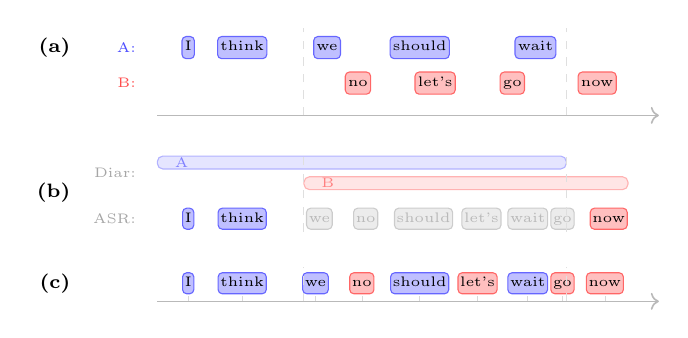
\begin{tikzpicture}[
    xscale=0.98,
    yscale=0.82,
    spkA/.style={fill=blue!25, draw=blue!60, rounded corners=1.5pt, minimum height=0.28cm, inner sep=1pt, font=\tiny\strut},
    spkB/.style={fill=red!25, draw=red!60, rounded corners=1.5pt, minimum height=0.28cm, inner sep=1pt, font=\tiny\strut},
    spkAt/.style={fill=blue!25, draw=blue!60, rounded corners=1.5pt, minimum height=0.26cm, inner sep=0.8pt, font=\tiny\strut},
    spkBt/.style={fill=red!25, draw=red!60, rounded corners=1.5pt, minimum height=0.26cm, inner sep=0.8pt, font=\tiny\strut},
    amb/.style={fill=gray!15, draw=gray!40, rounded corners=1.5pt, minimum height=0.24cm, inner sep=0.8pt, font=\tiny\strut, text=gray!55},
    timeline/.style={->, semithick, gray!55},
    lbl/.style={font=\scriptsize\bfseries, anchor=east},
]

% ---- (a) Ground truth ----
\node[lbl] at (-0.7, 2.6) {(a)};

\node[spkA] at (0.7, 2.6) {I};
\node[spkA] at (1.4, 2.6) {think};
\node[spkA] at (2.5, 2.6) {we};
\node[spkA] at (3.7, 2.6) {should};
\node[spkA] at (5.2, 2.6) {wait};

\node[spkB] at (2.9, 2.05) {no};
\node[spkB] at (3.9, 2.05) {let's};
\node[spkB] at (4.9, 2.05) {go};
\node[spkB] at (6.0, 2.05) {now};

\node[font=\tiny, blue!70, anchor=east] at (0.15, 2.6) {A:};
\node[font=\tiny, red!70, anchor=east] at (0.15, 2.05) {B:};

\draw[timeline] (0.3, 1.55) -- (6.8, 1.55);
\draw[dashed, gray!25, thin] (2.2, 1.55) -- (2.2, 2.9);
\draw[dashed, gray!25, thin] (5.6, 1.55) -- (5.6, 2.9);


% ---- (b) Cascade ----
\node[lbl] at (-0.7, 0.35) {(b)};

\draw[fill=blue!10, draw=blue!30, rounded corners=2pt] (0.3, 0.72) rectangle (5.6, 0.92);
\node[font=\tiny, blue!50, anchor=west] at (0.4, 0.82) {A};
\draw[fill=red!10, draw=red!30, rounded corners=2pt] (2.2, 0.4) rectangle (6.4, 0.6);
\node[font=\tiny, red!50, anchor=west] at (2.3, 0.5) {B};
\node[font=\tiny, gray!70, anchor=east] at (0.15, 0.66) {Diar:};

\node[font=\tiny, gray!70, anchor=east] at (0.15, -0.05) {ASR:};
\node[spkAt] at (0.7, -0.05) {I};
\node[spkAt] at (1.4, -0.05) {think};
\node[amb] at (2.4, -0.05) {we};
\node[amb] at (3.0, -0.05) {no};
\node[amb] at (3.75, -0.05) {should};
\node[amb] at (4.5, -0.05) {let's};
\node[amb] at (5.1, -0.05) {wait};
\node[amb] at (5.55, -0.05) {go};
\node[spkBt] at (6.15, -0.05) {now};

\draw[dashed, gray!25, thin] (2.2, -0.25) -- (2.2, 1.0);
\draw[dashed, gray!25, thin] (5.6, -0.25) -- (5.6, 1.0);


% ---- (c) Shuffle ----
\node[lbl] at (-0.7, -1.05) {(c)};

\node[spkAt] at (0.7, -1.05) {I};
\node[spkAt] at (1.4, -1.05) {think};
\node[spkAt] at (2.35, -1.05) {we};
\node[spkBt] at (2.95, -1.05) {no};
\node[spkAt] at (3.7, -1.05) {should};
\node[spkBt] at (4.45, -1.05) {let's};
\node[spkAt] at (5.1, -1.05) {wait};
\node[spkBt] at (5.55, -1.05) {go};
\node[spkBt] at (6.1, -1.05) {now};

\foreach \x in {0.7, 1.4, 2.35, 2.95, 3.7, 4.45, 5.1, 5.55, 6.1} {
    \draw[gray!30, very thin] (\x, -1.25) -- (\x, -1.33);
}
\draw[timeline] (0.3, -1.33) -- (6.8, -1.33);

\draw[dashed, gray!25, thin] (2.2, -1.33) -- (2.2, -0.8);
\draw[dashed, gray!25, thin] (5.6, -1.33) -- (5.6, -0.8);

\end{tikzpicture}
\caption{%
Word-level speaker attribution in overlapped speech.
\textbf{(a)}~Ground truth: speakers A (\textcolor{blue!60}{blue}) and B (\textcolor{red!60}{red}) produce concurrent tokens with partial overlap (dashed).
\textbf{(b)}~Cascade: diarization detects both speakers as active, but all ASR words in the overlap are ambiguous (gray) since both segments cover the same time.
\textbf{(c)}~Shuffle: the Viterbi path produces an interleaved, time-aligned, speaker-attributed sequence.
}
\label{fig:overlapped_attribution}
\vspace{-4mm}
\end{figure}

% Speaker diariazation, i.e., ``who spoke when,'' partially solves this task.
% %However, multi-talker alignment deals with speaker attribution of labels, not frames. In non-overlapped speech, these are equivalent problems -- one can decode each speaker specific segment and trivially assign all decoded tokens to the speaker of that segment. 
% %Conversely, if one can decode a single-speaker segment of speech and assign the decoded tokens to a speaker, e.g., by using a language model (LM) to detect switch points, then the speech is effectively diarized.
% In overlapped speech, however, frame-level activity does not uniquely determine the attribution of linguistic events and can result in combinatorially many ways of attributing tokens to speakers. 
% % Recent work addressing this problem has used serialized output training (SOT)~\cite{}, or iterative target speaker decoding to handle overlapped speech. However, these approaches often rely on a separate diarization system and do not easily support fine-grained alignment similar to traditional Viterbi-based alignment in HMM-GMM, CTC, or Transducer models.  
% % Furthermore, the most egregious ASR errors in multi-talker ASR come from assigning recognized output to the wrong speaker. In the case of cpWER~\cite{}, for example, the mis-attributed tokens count both as insertions with respect to the wrongly hypothesized speaker, and also as deletions with respect to the missed reference speaker, even if the hypothesized transcript is correct. Fixing such errors has the potential to dramatically improve multi-talker ASR performance.
% We therefore treat diarization as the task of assigning speakers to temporally localized labels. This directly answers the question ``who produced which label'' and since each label can still be approximately mapped to frame-level activity, it also solves the problem of ``who spoke when.'' Furthermore, our approach enables transcript conditioned diarization via alignment of audio to a set of transcripts. We therefore shift the problem from frame-level diarization to label synchronous diarization by modeling overlapped speech using shuffles as in \cite{wiesner2026modeling}, whose formulation unifies the treatment of overlapped and non-overlapped speech and enables one-pass multi-talker forced alignment. We demonstrate our approach on the AMI \cite{} and NOTSOFAR \cite{} datasets. %We also show the speaker attribution performance in terms of word diarization error rate (WDER) and diarization error rate of the speaker attribution component of the shuffle models, which has not been previously explored. The 
%---------------------
% Many multi-talker automatic speech recognition (ASR) systems require word-level timing information for training. In token-level serialized output training (t-SOT)~\cite{kanda22_interspeech} timing is required to construct the training targets in the correct order; the diarization-conditioned Whisper (DiCoW) family~\cite{polok2026dicow} requires timestamps to prepare supervisions for the 30\,s chunks used to fine-tune Whisper for multi-talker ASR. Obtaining such transcripts is difficult. Word-level timestamps in corpora such as AMI~\cite{carletta2005ami} and NOTSOFAR-1 (NSF1)~\cite{vinnikov2024notsofar} exist only because each speaker was recorded on a separate close-talk or throat microphone, to which well-established single-speaker forced alignment~\cite{mcauliffe2017montreal} can be applied. Most multi-talker audio has a transcript but no per-speaker channel, and, to our knowledge, no single technique produces speaker-attributed word timing from the mixture alone. 
% Some large-scale text-to-speech data pipelines~\cite{he2024emilia, jung2026sommelier} instead apply source separation and diarization to obtain single-speaker segments that a standard aligner can process. This is effective on web audio with limited overlap, but in far-field conversational scenatios neural speech separation degrades and ceases to be effective, in particular as a front-end for ASR~\cite{cornell2025recent}. 

% Forced alignment of single-speaker audio is a well-established problem. HMM-based aligners such as MFA~\cite{mcauliffe2017montreal, povey2011kaldi}, CTC-based aligners~\cite{huang2024less, rastorgueva2023nfa, bain2023whisperx} and recent saliency-based approaches~\cite{zeyer2026gradient} all model one token sequence and one active speaker per frame. Since Viterbi search through a transcript graph does not scale to long recordings, they segment the audio with voice activity detection (VAD) or a first decoding pass, possibly biased towards the transcript ~\cite{lamel2002lightly, manohar2017jhu}, and align each segment separately~\cite{moreno1998recursive, katsamanis2011sailalign}. This strategy requires either silent regions at which to segment or a first pass that is accurate enough to provide anchors. The alternative is to keep the exact search and reduce its memory, for instance by check-pointing the Viterbi algorithm~\cite{grice1997reduced} or by pruning it to a band~\cite{kuang2022pruned}. 
% Moreover, even when close-talk microphones exist, overlapped speech remains an obstacle. On mixed-headset AMI recordings, MFA produced an alignment for only 5 of 16 meetings~\cite{rastorgueva2023nfa}, and the aligners that succeeded did so on a transcript in which all speakers' words were concatenated into a single sequence. Their output therefore carries no speaker attribution, which most applications require: localizing a token (phoneme, byte-pair unit, word or syllable) in time solves only part of the multi-talker alignment problem (Fig.~\ref{fig:overlapped_attribution}).

% \begin{figure}[t]
\centering
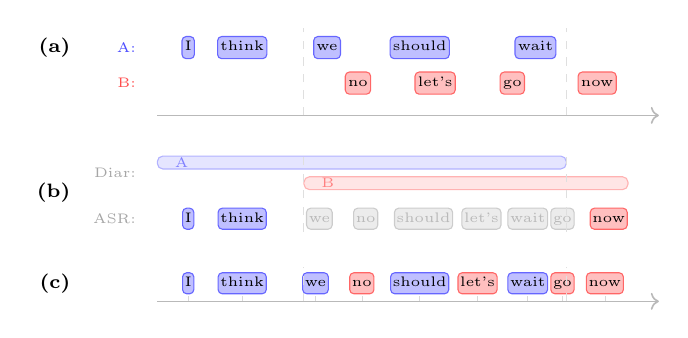
\begin{tikzpicture}[
    xscale=0.98,
    yscale=0.82,
    spkA/.style={fill=blue!25, draw=blue!60, rounded corners=1.5pt, minimum height=0.28cm, inner sep=1pt, font=\tiny\strut},
    spkB/.style={fill=red!25, draw=red!60, rounded corners=1.5pt, minimum height=0.28cm, inner sep=1pt, font=\tiny\strut},
    spkAt/.style={fill=blue!25, draw=blue!60, rounded corners=1.5pt, minimum height=0.26cm, inner sep=0.8pt, font=\tiny\strut},
    spkBt/.style={fill=red!25, draw=red!60, rounded corners=1.5pt, minimum height=0.26cm, inner sep=0.8pt, font=\tiny\strut},
    amb/.style={fill=gray!15, draw=gray!40, rounded corners=1.5pt, minimum height=0.24cm, inner sep=0.8pt, font=\tiny\strut, text=gray!55},
    timeline/.style={->, semithick, gray!55},
    lbl/.style={font=\scriptsize\bfseries, anchor=east},
]

% ---- (a) Ground truth ----
\node[lbl] at (-0.7, 2.6) {(a)};

\node[spkA] at (0.7, 2.6) {I};
\node[spkA] at (1.4, 2.6) {think};
\node[spkA] at (2.5, 2.6) {we};
\node[spkA] at (3.7, 2.6) {should};
\node[spkA] at (5.2, 2.6) {wait};

\node[spkB] at (2.9, 2.05) {no};
\node[spkB] at (3.9, 2.05) {let's};
\node[spkB] at (4.9, 2.05) {go};
\node[spkB] at (6.0, 2.05) {now};

\node[font=\tiny, blue!70, anchor=east] at (0.15, 2.6) {A:};
\node[font=\tiny, red!70, anchor=east] at (0.15, 2.05) {B:};

\draw[timeline] (0.3, 1.55) -- (6.8, 1.55);
\draw[dashed, gray!25, thin] (2.2, 1.55) -- (2.2, 2.9);
\draw[dashed, gray!25, thin] (5.6, 1.55) -- (5.6, 2.9);


% ---- (b) Cascade ----
\node[lbl] at (-0.7, 0.35) {(b)};

\draw[fill=blue!10, draw=blue!30, rounded corners=2pt] (0.3, 0.72) rectangle (5.6, 0.92);
\node[font=\tiny, blue!50, anchor=west] at (0.4, 0.82) {A};
\draw[fill=red!10, draw=red!30, rounded corners=2pt] (2.2, 0.4) rectangle (6.4, 0.6);
\node[font=\tiny, red!50, anchor=west] at (2.3, 0.5) {B};
\node[font=\tiny, gray!70, anchor=east] at (0.15, 0.66) {Diar:};

\node[font=\tiny, gray!70, anchor=east] at (0.15, -0.05) {ASR:};
\node[spkAt] at (0.7, -0.05) {I};
\node[spkAt] at (1.4, -0.05) {think};
\node[amb] at (2.4, -0.05) {we};
\node[amb] at (3.0, -0.05) {no};
\node[amb] at (3.75, -0.05) {should};
\node[amb] at (4.5, -0.05) {let's};
\node[amb] at (5.1, -0.05) {wait};
\node[amb] at (5.55, -0.05) {go};
\node[spkBt] at (6.15, -0.05) {now};

\draw[dashed, gray!25, thin] (2.2, -0.25) -- (2.2, 1.0);
\draw[dashed, gray!25, thin] (5.6, -0.25) -- (5.6, 1.0);


% ---- (c) Shuffle ----
\node[lbl] at (-0.7, -1.05) {(c)};

\node[spkAt] at (0.7, -1.05) {I};
\node[spkAt] at (1.4, -1.05) {think};
\node[spkAt] at (2.35, -1.05) {we};
\node[spkBt] at (2.95, -1.05) {no};
\node[spkAt] at (3.7, -1.05) {should};
\node[spkBt] at (4.45, -1.05) {let's};
\node[spkAt] at (5.1, -1.05) {wait};
\node[spkBt] at (5.55, -1.05) {go};
\node[spkBt] at (6.1, -1.05) {now};

\foreach \x in {0.7, 1.4, 2.35, 2.95, 3.7, 4.45, 5.1, 5.55, 6.1} {
    \draw[gray!30, very thin] (\x, -1.25) -- (\x, -1.33);
}
\draw[timeline] (0.3, -1.33) -- (6.8, -1.33);

\draw[dashed, gray!25, thin] (2.2, -1.33) -- (2.2, -0.8);
\draw[dashed, gray!25, thin] (5.6, -1.33) -- (5.6, -0.8);

\end{tikzpicture}
\caption{%
Word-level speaker attribution in overlapped speech.
\textbf{(a)}~Ground truth: speakers A (\textcolor{blue!60}{blue}) and B (\textcolor{red!60}{red}) produce concurrent tokens with partial overlap (dashed).
\textbf{(b)}~Cascade: diarization detects both speakers as active, but all ASR words in the overlap are ambiguous (gray) since both segments cover the same time.
\textbf{(c)}~Shuffle: the Viterbi path produces an interleaved, time-aligned, speaker-attributed sequence.
}
\label{fig:overlapped_attribution}
\vspace{-4mm}
\end{figure}

% In~\cite{wiesner2026modeling} we recently proposed constructing alignment graphs from the shuffle product of multi-talker transcripts. The shuffle formulation treats overlapped and non-overlapped speech uniformly and permits multi-talker forced alignment in a single Viterbi pass, and we reported results on synthetic 30\,s mixtures of two and three speakers. That work has however two limitations that this paper addresses. First, applied without modification, the method does not scale to longer recordings or to more speakers, and cannot be used on long-form conversational speech such as meetings~\cite{carletta2005ami, vinnikov2024notsofar, cornell2025recent}. Second, it assumed speaker-attributed transcripts, whereas in practice transcripts often carry utterance boundaries but no speaker labels. Speaker diarization, which determines who spoke when, does not resolve this case: in overlapped speech, frame-level activity does not determine which speaker produced which token, and the number of consistent assignments grows combinatorially. Attributing utterances to speakers is an instance of the speaker partitioning problem of Br\"ummer and de Villiers~\cite{brummer2010speaker}, whose solution space grows with the Bell numbers and which clustering methods such as VBx~\cite{landini2022bayesian} solve approximately from acoustics alone. We instead treat diarization as the assignment of speakers to temporally localized labels, which specifies which speaker produced each label and, since each label maps to a set of frames, also who spoke when. This label-synchronous view permits transcript-conditioned diarization: the audio is aligned to a set of transcripts without speaker labels, and the speaker partition is then scored under the acoustic model given the token alignment.

% The contributions of this paper are: (i) a set of inference techniques that make shuffle-based alignment of long recordings with many speakers feasible on a single GPU, each evaluated in an ablation (Section~\ref{sec:longform}); (ii) a method for speaker attribution of transcripts without speaker labels, formulated as token alignment followed by a search over speaker partitions using the frame-level speaker posteriors of a speaker-attributed shuffle model (Section~\ref{sec:attribution}); and (iii) an out-of-domain evaluation on AMI and NSF1 of models trained only on synthetic and web-scraped data, which are publicly released.
%----------------------------
Many multi-talker automatic speech recognition (ASR) systems require word-level timing information for training. Token-level serialized output training (t-SOT)~\cite{kanda22_interspeech} uses timing to order training targets, while diarization-conditioned Whisper (DiCoW)~\cite{polok2026dicow} requires timestamps to prepare supervision for the 30\,s chunks used to fine-tune Whisper. Word-level timestamps are difficult to obtain. In corpora such as AMI~\cite{carletta2005ami} and NOTSOFAR-1 (NSF)~\cite{vinnikov2024notsofar} they exist because a separate close-talk or throat microphone recorded each speaker, enabling single-speaker forced alignment~\cite{mcauliffe2017montreal}. Most multi-talker recordings separate speaker channels and, to our knowledge, no single technique produces speaker-attributed word timing directly from the mixture. Large-scale text-to-speech pipelines~\cite{he2024emilia, jung2026sommelier} cascade source separation and diarization to obtain single-speaker segments for alignment, but separation degrades in far-field conversational speech, particularly as an ASR front end~\cite{cornell2025recent}.

Forced alignment of single-speaker audio is well established. HMM-based aligners such as MFA~\cite{mcauliffe2017montreal, povey2011kaldi}, connectionist temporal classification (CTC)-based aligners~\cite{huang2024less, rastorgueva2023nfa, bain2023whisperx},
and recent saliency-based approaches~\cite{zeyer2026gradient} assume one token sequence and one active speaker per frame. Because exact Viterbi search through long transcript graphs is memory intensive, long recordings are commonly segmented using VAD or a first decoding pass, possibly biased toward the transcript~\cite{ manohar2017jhu}, and aligned segment by segment~\cite{moreno1998recursive, katsamanis2011sailalign}. This requires either suitable silence boundaries or sufficiently accurate anchors. Alternatives retain the exact search while reducing memory, for example through Viterbi checkpointing~\cite{grice1997reduced} or band pruning~\cite{kuang2022pruned}. Overlap is problematic even with close-talk microphones: on mixed-headset AMI recordings, MFA aligned only 5 of 16 meetings~\cite{rastorgueva2023nfa}. Successful aligners operated on a single sequence formed by concatenating all speakers' words, but outputs then lack speaker attribution: localizing a token in time is only one part of multi-talker alignment (Figure ~\ref{fig:overlapped_attribution}).

\begin{figure}[t]
\centering
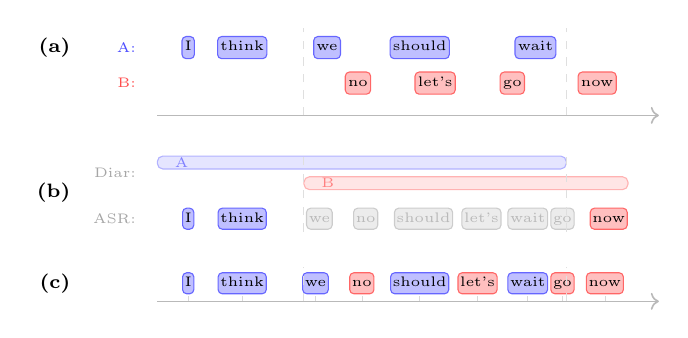
\begin{tikzpicture}[
    xscale=0.98,
    yscale=0.82,
    spkA/.style={fill=blue!25, draw=blue!60, rounded corners=1.5pt, minimum height=0.28cm, inner sep=1pt, font=\tiny\strut},
    spkB/.style={fill=red!25, draw=red!60, rounded corners=1.5pt, minimum height=0.28cm, inner sep=1pt, font=\tiny\strut},
    spkAt/.style={fill=blue!25, draw=blue!60, rounded corners=1.5pt, minimum height=0.26cm, inner sep=0.8pt, font=\tiny\strut},
    spkBt/.style={fill=red!25, draw=red!60, rounded corners=1.5pt, minimum height=0.26cm, inner sep=0.8pt, font=\tiny\strut},
    amb/.style={fill=gray!15, draw=gray!40, rounded corners=1.5pt, minimum height=0.24cm, inner sep=0.8pt, font=\tiny\strut, text=gray!55},
    timeline/.style={->, semithick, gray!55},
    lbl/.style={font=\scriptsize\bfseries, anchor=east},
]

% ---- (a) Ground truth ----
\node[lbl] at (-0.7, 2.6) {(a)};

\node[spkA] at (0.7, 2.6) {I};
\node[spkA] at (1.4, 2.6) {think};
\node[spkA] at (2.5, 2.6) {we};
\node[spkA] at (3.7, 2.6) {should};
\node[spkA] at (5.2, 2.6) {wait};

\node[spkB] at (2.9, 2.05) {no};
\node[spkB] at (3.9, 2.05) {let's};
\node[spkB] at (4.9, 2.05) {go};
\node[spkB] at (6.0, 2.05) {now};

\node[font=\tiny, blue!70, anchor=east] at (0.15, 2.6) {A:};
\node[font=\tiny, red!70, anchor=east] at (0.15, 2.05) {B:};

\draw[timeline] (0.3, 1.55) -- (6.8, 1.55);
\draw[dashed, gray!25, thin] (2.2, 1.55) -- (2.2, 2.9);
\draw[dashed, gray!25, thin] (5.6, 1.55) -- (5.6, 2.9);


% ---- (b) Cascade ----
\node[lbl] at (-0.7, 0.35) {(b)};

\draw[fill=blue!10, draw=blue!30, rounded corners=2pt] (0.3, 0.72) rectangle (5.6, 0.92);
\node[font=\tiny, blue!50, anchor=west] at (0.4, 0.82) {A};
\draw[fill=red!10, draw=red!30, rounded corners=2pt] (2.2, 0.4) rectangle (6.4, 0.6);
\node[font=\tiny, red!50, anchor=west] at (2.3, 0.5) {B};
\node[font=\tiny, gray!70, anchor=east] at (0.15, 0.66) {Diar:};

\node[font=\tiny, gray!70, anchor=east] at (0.15, -0.05) {ASR:};
\node[spkAt] at (0.7, -0.05) {I};
\node[spkAt] at (1.4, -0.05) {think};
\node[amb] at (2.4, -0.05) {we};
\node[amb] at (3.0, -0.05) {no};
\node[amb] at (3.75, -0.05) {should};
\node[amb] at (4.5, -0.05) {let's};
\node[amb] at (5.1, -0.05) {wait};
\node[amb] at (5.55, -0.05) {go};
\node[spkBt] at (6.15, -0.05) {now};

\draw[dashed, gray!25, thin] (2.2, -0.25) -- (2.2, 1.0);
\draw[dashed, gray!25, thin] (5.6, -0.25) -- (5.6, 1.0);


% ---- (c) Shuffle ----
\node[lbl] at (-0.7, -1.05) {(c)};

\node[spkAt] at (0.7, -1.05) {I};
\node[spkAt] at (1.4, -1.05) {think};
\node[spkAt] at (2.35, -1.05) {we};
\node[spkBt] at (2.95, -1.05) {no};
\node[spkAt] at (3.7, -1.05) {should};
\node[spkBt] at (4.45, -1.05) {let's};
\node[spkAt] at (5.1, -1.05) {wait};
\node[spkBt] at (5.55, -1.05) {go};
\node[spkBt] at (6.1, -1.05) {now};

\foreach \x in {0.7, 1.4, 2.35, 2.95, 3.7, 4.45, 5.1, 5.55, 6.1} {
    \draw[gray!30, very thin] (\x, -1.25) -- (\x, -1.33);
}
\draw[timeline] (0.3, -1.33) -- (6.8, -1.33);

\draw[dashed, gray!25, thin] (2.2, -1.33) -- (2.2, -0.8);
\draw[dashed, gray!25, thin] (5.6, -1.33) -- (5.6, -0.8);

\end{tikzpicture}
\caption{%
Word-level speaker attribution in overlapped speech.
\textbf{(a)}~Ground truth: speakers A (\textcolor{blue!60}{blue}) and B (\textcolor{red!60}{red}) produce concurrent tokens with partial overlap (dashed).
\textbf{(b)}~Cascade: diarization detects both speakers as active, but all ASR words in the overlap are ambiguous (gray) since both segments cover the same time.
\textbf{(c)}~Shuffle: the Viterbi path produces an interleaved, time-aligned, speaker-attributed sequence.
}
\label{fig:overlapped_attribution}
\vspace{-4mm}
\end{figure}

In~\cite{wiesner2026modeling} we proposed constructing alignment graphs from the shuffle product of multi-talker transcripts, treating overlapped and non-overlapped speech uniformly and enabling multi-talker forced alignment in a single Viterbi pass. We evaluated the approach on synthetic 30s mixtures of two and three speakers, but it has two limitations addressed here. First, without modification it does not easily scale to longer recordings or more speakers, preventing application to meeting-style speech~\cite{carletta2005ami, vinnikov2024notsofar, cornell2025recent}. Second, it assumes speaker-attributed transcripts, whereas practical transcripts often provide utterance boundaries but no speaker labels. Speaker diarization alone does not resolve this ambiguity in overlapped speech: frame-level activity does not uniquely determine who produced each token.

Assigning utterances to speakers is an instance of the speaker partitioning problem~\cite{brummer2010speaker}, whose solution space grows with the Bell numbers and which clustering methods such as VBx~\cite{landini2022bayesian} solve approximately from acoustics alone. Similar to \cite{9746225},  we instead view diarization as assigning temporally localized labels to speakers. This permits transcript-conditioned diarization, similar in spirit to \cite{shafey19_interspeech, park19_interspeech}: the audio is first aligned to transcripts without speaker labels, after which speaker partitions are scored under the acoustic model given the token alignment.

The contributions of this paper are: (i) inference techniques that make shuffle-based alignment of long recordings with many speakers feasible on a single GPU, evaluated by ablation (Section~\ref{sec:results_longform}); (ii) speaker attribution for transcripts without speaker labels, formulated as token alignment followed by search over speaker partitions using frame-level speaker posteriors from a speaker-attributed shuffle model (Section~\ref{sec:speaker_attribution}); and (iii) out-of-domain evaluation of publicly released models trained only on synthetic and web-scraped data on the AMI and NSF1 single distant microphone (SDM) condition.
%
%\section{Introduction}
%% Many modern multi-talker Automatic Speech Recognition (ASR) systems require world-level timing information for training. In token-level Serialized Output Training \cite{kanda22_interspeech} (t-SOT) timing is required for constructing the training targets in the correct order; the Diarization Conditioned Whisper (DiCoW) model family \cite{polok2026dicow} requires time stamps to prepare supervisions for the 30s audio chunks used for fine-tuning Whisper, which it re-purposes for multi-talker ASR.

% Unfortunately, obtaining time-stamped transcripts is difficult. World-level time-stamps in common multi-talker ASR corpora, such as AMI \cite{carletta2005ami}, and NOTSOFAR-1 (NSF1) \cite{vinnikov2024notsofar}, are possible thanks to an expensive data collection procedures involving separate close-talk, or throat microphones. These speaker-specific channels enable the use of well-established forced alignment methods \cite{mcauliffe2017montreal} to retrieve time-stamped transcripts. Some corpora are even manually annotated for timing information \cite{pitt2005buckeye, garofolo1993timit}.

% Standard forced alignment relies on Viterbi search through a transcript graph in which each transition represents the time at which a label is produced. However, this procedure does not scale well to long recordings. Common approaches \cite{katsamanis2011sailalign, checkpointing, CTC_align, mcauliffe2017montreal} for long-form alignment, such as \textsc{Sail}, \textsc{CTC align}, or \textsc{kaldi}-based recipes \cite{povey2011kaldi}, use an initial step of voice activity detection (VAD) or first-pass decoding (possibly transcript-biased decoding \cite{biased_LMs}) to create more manageable segments. However, this approach struggles in multi-talker scenarios as continuous conversation means there are few regions of silence since at least one person is usually speaking. Forced alignment is also not well equipped to deal with overlapped speech, and forced alignment packages, such as the Montreal Forced Aligner (MFA), do not work well in this scenario. Even when speech can be aligned, it is not very useful without speaker attribution (see Fig. \ref{fig:overlapped_attribution}).
% %e.g., A: How old are you? B: twenty C: eight, has a very different meaning from, A: How old are you? B: twenty-eight, or A: How old are you? twenty-eight?

% We recently proposed using alignment graphs constructed from the shuffle product of multi-talker transcripts \cite{wiesner2026modeling}, and showed some promising preliminary results on synthetic 2 and 3 speaker 30\,s audio clips. However, the method, at least when applied naively, does not scale to longer audio recordings or to more speakers, making it unsuitable for alignment of long-form conversational speech such as meeting scenarios~\cite{carletta2005ami, vinnikov2024notsofar, cornell2025recent}. Furthermore, in multi-talker forced alignment, localizing a token (phoneme, byte-pair encoding-unit, word, or syllable) in time only partially solves the alignment problem as also speaker attribution is essential. In \cite{wiesner2026modeling} we did not  explore this problem or to what extent alignment is possible without speaker attributed transcripts.

% \begin{figure}[t]
\centering
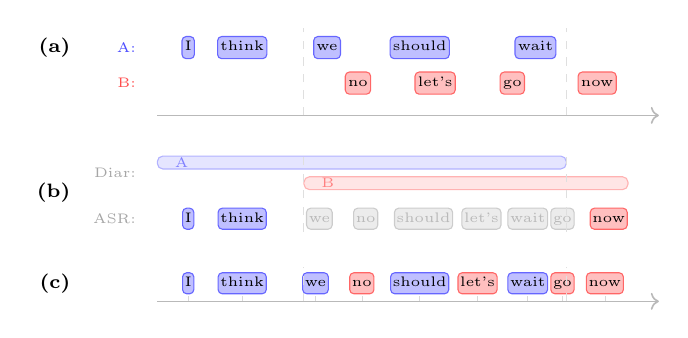
\begin{tikzpicture}[
    xscale=0.98,
    yscale=0.82,
    spkA/.style={fill=blue!25, draw=blue!60, rounded corners=1.5pt, minimum height=0.28cm, inner sep=1pt, font=\tiny\strut},
    spkB/.style={fill=red!25, draw=red!60, rounded corners=1.5pt, minimum height=0.28cm, inner sep=1pt, font=\tiny\strut},
    spkAt/.style={fill=blue!25, draw=blue!60, rounded corners=1.5pt, minimum height=0.26cm, inner sep=0.8pt, font=\tiny\strut},
    spkBt/.style={fill=red!25, draw=red!60, rounded corners=1.5pt, minimum height=0.26cm, inner sep=0.8pt, font=\tiny\strut},
    amb/.style={fill=gray!15, draw=gray!40, rounded corners=1.5pt, minimum height=0.24cm, inner sep=0.8pt, font=\tiny\strut, text=gray!55},
    timeline/.style={->, semithick, gray!55},
    lbl/.style={font=\scriptsize\bfseries, anchor=east},
]

% ---- (a) Ground truth ----
\node[lbl] at (-0.7, 2.6) {(a)};

\node[spkA] at (0.7, 2.6) {I};
\node[spkA] at (1.4, 2.6) {think};
\node[spkA] at (2.5, 2.6) {we};
\node[spkA] at (3.7, 2.6) {should};
\node[spkA] at (5.2, 2.6) {wait};

\node[spkB] at (2.9, 2.05) {no};
\node[spkB] at (3.9, 2.05) {let's};
\node[spkB] at (4.9, 2.05) {go};
\node[spkB] at (6.0, 2.05) {now};

\node[font=\tiny, blue!70, anchor=east] at (0.15, 2.6) {A:};
\node[font=\tiny, red!70, anchor=east] at (0.15, 2.05) {B:};

\draw[timeline] (0.3, 1.55) -- (6.8, 1.55);
\draw[dashed, gray!25, thin] (2.2, 1.55) -- (2.2, 2.9);
\draw[dashed, gray!25, thin] (5.6, 1.55) -- (5.6, 2.9);


% ---- (b) Cascade ----
\node[lbl] at (-0.7, 0.35) {(b)};

\draw[fill=blue!10, draw=blue!30, rounded corners=2pt] (0.3, 0.72) rectangle (5.6, 0.92);
\node[font=\tiny, blue!50, anchor=west] at (0.4, 0.82) {A};
\draw[fill=red!10, draw=red!30, rounded corners=2pt] (2.2, 0.4) rectangle (6.4, 0.6);
\node[font=\tiny, red!50, anchor=west] at (2.3, 0.5) {B};
\node[font=\tiny, gray!70, anchor=east] at (0.15, 0.66) {Diar:};

\node[font=\tiny, gray!70, anchor=east] at (0.15, -0.05) {ASR:};
\node[spkAt] at (0.7, -0.05) {I};
\node[spkAt] at (1.4, -0.05) {think};
\node[amb] at (2.4, -0.05) {we};
\node[amb] at (3.0, -0.05) {no};
\node[amb] at (3.75, -0.05) {should};
\node[amb] at (4.5, -0.05) {let's};
\node[amb] at (5.1, -0.05) {wait};
\node[amb] at (5.55, -0.05) {go};
\node[spkBt] at (6.15, -0.05) {now};

\draw[dashed, gray!25, thin] (2.2, -0.25) -- (2.2, 1.0);
\draw[dashed, gray!25, thin] (5.6, -0.25) -- (5.6, 1.0);


% ---- (c) Shuffle ----
\node[lbl] at (-0.7, -1.05) {(c)};

\node[spkAt] at (0.7, -1.05) {I};
\node[spkAt] at (1.4, -1.05) {think};
\node[spkAt] at (2.35, -1.05) {we};
\node[spkBt] at (2.95, -1.05) {no};
\node[spkAt] at (3.7, -1.05) {should};
\node[spkBt] at (4.45, -1.05) {let's};
\node[spkAt] at (5.1, -1.05) {wait};
\node[spkBt] at (5.55, -1.05) {go};
\node[spkBt] at (6.1, -1.05) {now};

\foreach \x in {0.7, 1.4, 2.35, 2.95, 3.7, 4.45, 5.1, 5.55, 6.1} {
    \draw[gray!30, very thin] (\x, -1.25) -- (\x, -1.33);
}
\draw[timeline] (0.3, -1.33) -- (6.8, -1.33);

\draw[dashed, gray!25, thin] (2.2, -1.33) -- (2.2, -0.8);
\draw[dashed, gray!25, thin] (5.6, -1.33) -- (5.6, -0.8);

\end{tikzpicture}
\caption{%
Word-level speaker attribution in overlapped speech.
\textbf{(a)}~Ground truth: speakers A (\textcolor{blue!60}{blue}) and B (\textcolor{red!60}{red}) produce concurrent tokens with partial overlap (dashed).
\textbf{(b)}~Cascade: diarization detects both speakers as active, but all ASR words in the overlap are ambiguous (gray) since both segments cover the same time.
\textbf{(c)}~Shuffle: the Viterbi path produces an interleaved, time-aligned, speaker-attributed sequence.
}
\label{fig:overlapped_attribution}
\vspace{-4mm}
\end{figure}

% Speaker diariazation, i.e., ``who spoke when,'' partially solves this task.
% %However, multi-talker alignment deals with speaker attribution of labels, not frames. In non-overlapped speech, these are equivalent problems -- one can decode each speaker specific segment and trivially assign all decoded tokens to the speaker of that segment. 
% %Conversely, if one can decode a single-speaker segment of speech and assign the decoded tokens to a speaker, e.g., by using a language model (LM) to detect switch points, then the speech is effectively diarized.
% In overlapped speech, however, frame-level activity does not uniquely determine the attribution of linguistic events and can result in combinatorially many ways of attributing tokens to speakers. 
% % Recent work addressing this problem has used serialized output training (SOT)~\cite{}, or iterative target speaker decoding to handle overlapped speech. However, these approaches often rely on a separate diarization system and do not easily support fine-grained alignment similar to traditional Viterbi-based alignment in HMM-GMM, CTC, or Transducer models.  
% % Furthermore, the most egregious ASR errors in multi-talker ASR come from assigning recognized output to the wrong speaker. In the case of cpWER~\cite{}, for example, the mis-attributed tokens count both as insertions with respect to the wrongly hypothesized speaker, and also as deletions with respect to the missed reference speaker, even if the hypothesized transcript is correct. Fixing such errors has the potential to dramatically improve multi-talker ASR performance.
% We therefore treat diarization as the task of assigning speakers to temporally localized labels. This directly answers the question ``who produced which label'' and since each label can still be approximately mapped to frame-level activity, it also solves the problem of ``who spoke when.'' Furthermore, our approach enables transcript conditioned diarization via alignment of audio to a set of transcripts. We therefore shift the problem from frame-level diarization to label synchronous diarization by modeling overlapped speech using shuffles as in \cite{wiesner2026modeling}, whose formulation unifies the treatment of overlapped and non-overlapped speech and enables one-pass multi-talker forced alignment. We demonstrate our approach on the AMI \cite{} and NOTSOFAR \cite{} datasets. %We also show the speaker attribution performance in terms of word diarization error rate (WDER) and diarization error rate of the speaker attribution component of the shuffle models, which has not been previously explored. The 
%---------------------
% Many multi-talker automatic speech recognition (ASR) systems require word-level timing information for training. In token-level serialized output training (t-SOT)~\cite{kanda22_interspeech} timing is required to construct the training targets in the correct order; the diarization-conditioned Whisper (DiCoW) family~\cite{polok2026dicow} requires timestamps to prepare supervisions for the 30\,s chunks used to fine-tune Whisper for multi-talker ASR. Obtaining such transcripts is difficult. Word-level timestamps in corpora such as AMI~\cite{carletta2005ami} and NOTSOFAR-1 (NSF1)~\cite{vinnikov2024notsofar} exist only because each speaker was recorded on a separate close-talk or throat microphone, to which well-established single-speaker forced alignment~\cite{mcauliffe2017montreal} can be applied. Most multi-talker audio has a transcript but no per-speaker channel, and, to our knowledge, no single technique produces speaker-attributed word timing from the mixture alone. 
% Some large-scale text-to-speech data pipelines~\cite{he2024emilia, jung2026sommelier} instead apply source separation and diarization to obtain single-speaker segments that a standard aligner can process. This is effective on web audio with limited overlap, but in far-field conversational scenatios neural speech separation degrades and ceases to be effective, in particular as a front-end for ASR~\cite{cornell2025recent}. 

% Forced alignment of single-speaker audio is a well-established problem. HMM-based aligners such as MFA~\cite{mcauliffe2017montreal, povey2011kaldi}, CTC-based aligners~\cite{huang2024less, rastorgueva2023nfa, bain2023whisperx} and recent saliency-based approaches~\cite{zeyer2026gradient} all model one token sequence and one active speaker per frame. Since Viterbi search through a transcript graph does not scale to long recordings, they segment the audio with voice activity detection (VAD) or a first decoding pass, possibly biased towards the transcript ~\cite{lamel2002lightly, manohar2017jhu}, and align each segment separately~\cite{moreno1998recursive, katsamanis2011sailalign}. This strategy requires either silent regions at which to segment or a first pass that is accurate enough to provide anchors. The alternative is to keep the exact search and reduce its memory, for instance by check-pointing the Viterbi algorithm~\cite{grice1997reduced} or by pruning it to a band~\cite{kuang2022pruned}. 
% Moreover, even when close-talk microphones exist, overlapped speech remains an obstacle. On mixed-headset AMI recordings, MFA produced an alignment for only 5 of 16 meetings~\cite{rastorgueva2023nfa}, and the aligners that succeeded did so on a transcript in which all speakers' words were concatenated into a single sequence. Their output therefore carries no speaker attribution, which most applications require: localizing a token (phoneme, byte-pair unit, word or syllable) in time solves only part of the multi-talker alignment problem (Fig.~\ref{fig:overlapped_attribution}).

% \begin{figure}[t]
\centering
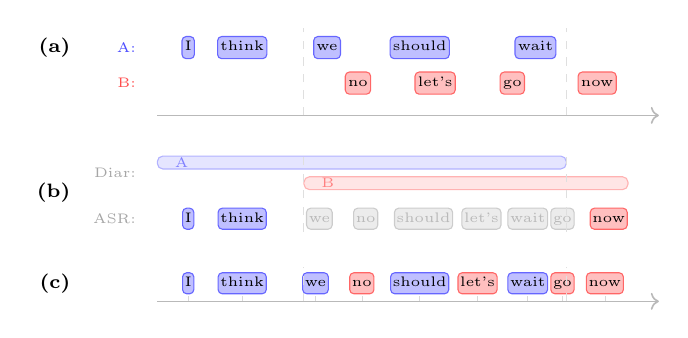
\begin{tikzpicture}[
    xscale=0.98,
    yscale=0.82,
    spkA/.style={fill=blue!25, draw=blue!60, rounded corners=1.5pt, minimum height=0.28cm, inner sep=1pt, font=\tiny\strut},
    spkB/.style={fill=red!25, draw=red!60, rounded corners=1.5pt, minimum height=0.28cm, inner sep=1pt, font=\tiny\strut},
    spkAt/.style={fill=blue!25, draw=blue!60, rounded corners=1.5pt, minimum height=0.26cm, inner sep=0.8pt, font=\tiny\strut},
    spkBt/.style={fill=red!25, draw=red!60, rounded corners=1.5pt, minimum height=0.26cm, inner sep=0.8pt, font=\tiny\strut},
    amb/.style={fill=gray!15, draw=gray!40, rounded corners=1.5pt, minimum height=0.24cm, inner sep=0.8pt, font=\tiny\strut, text=gray!55},
    timeline/.style={->, semithick, gray!55},
    lbl/.style={font=\scriptsize\bfseries, anchor=east},
]

% ---- (a) Ground truth ----
\node[lbl] at (-0.7, 2.6) {(a)};

\node[spkA] at (0.7, 2.6) {I};
\node[spkA] at (1.4, 2.6) {think};
\node[spkA] at (2.5, 2.6) {we};
\node[spkA] at (3.7, 2.6) {should};
\node[spkA] at (5.2, 2.6) {wait};

\node[spkB] at (2.9, 2.05) {no};
\node[spkB] at (3.9, 2.05) {let's};
\node[spkB] at (4.9, 2.05) {go};
\node[spkB] at (6.0, 2.05) {now};

\node[font=\tiny, blue!70, anchor=east] at (0.15, 2.6) {A:};
\node[font=\tiny, red!70, anchor=east] at (0.15, 2.05) {B:};

\draw[timeline] (0.3, 1.55) -- (6.8, 1.55);
\draw[dashed, gray!25, thin] (2.2, 1.55) -- (2.2, 2.9);
\draw[dashed, gray!25, thin] (5.6, 1.55) -- (5.6, 2.9);


% ---- (b) Cascade ----
\node[lbl] at (-0.7, 0.35) {(b)};

\draw[fill=blue!10, draw=blue!30, rounded corners=2pt] (0.3, 0.72) rectangle (5.6, 0.92);
\node[font=\tiny, blue!50, anchor=west] at (0.4, 0.82) {A};
\draw[fill=red!10, draw=red!30, rounded corners=2pt] (2.2, 0.4) rectangle (6.4, 0.6);
\node[font=\tiny, red!50, anchor=west] at (2.3, 0.5) {B};
\node[font=\tiny, gray!70, anchor=east] at (0.15, 0.66) {Diar:};

\node[font=\tiny, gray!70, anchor=east] at (0.15, -0.05) {ASR:};
\node[spkAt] at (0.7, -0.05) {I};
\node[spkAt] at (1.4, -0.05) {think};
\node[amb] at (2.4, -0.05) {we};
\node[amb] at (3.0, -0.05) {no};
\node[amb] at (3.75, -0.05) {should};
\node[amb] at (4.5, -0.05) {let's};
\node[amb] at (5.1, -0.05) {wait};
\node[amb] at (5.55, -0.05) {go};
\node[spkBt] at (6.15, -0.05) {now};

\draw[dashed, gray!25, thin] (2.2, -0.25) -- (2.2, 1.0);
\draw[dashed, gray!25, thin] (5.6, -0.25) -- (5.6, 1.0);


% ---- (c) Shuffle ----
\node[lbl] at (-0.7, -1.05) {(c)};

\node[spkAt] at (0.7, -1.05) {I};
\node[spkAt] at (1.4, -1.05) {think};
\node[spkAt] at (2.35, -1.05) {we};
\node[spkBt] at (2.95, -1.05) {no};
\node[spkAt] at (3.7, -1.05) {should};
\node[spkBt] at (4.45, -1.05) {let's};
\node[spkAt] at (5.1, -1.05) {wait};
\node[spkBt] at (5.55, -1.05) {go};
\node[spkBt] at (6.1, -1.05) {now};

\foreach \x in {0.7, 1.4, 2.35, 2.95, 3.7, 4.45, 5.1, 5.55, 6.1} {
    \draw[gray!30, very thin] (\x, -1.25) -- (\x, -1.33);
}
\draw[timeline] (0.3, -1.33) -- (6.8, -1.33);

\draw[dashed, gray!25, thin] (2.2, -1.33) -- (2.2, -0.8);
\draw[dashed, gray!25, thin] (5.6, -1.33) -- (5.6, -0.8);

\end{tikzpicture}
\caption{%
Word-level speaker attribution in overlapped speech.
\textbf{(a)}~Ground truth: speakers A (\textcolor{blue!60}{blue}) and B (\textcolor{red!60}{red}) produce concurrent tokens with partial overlap (dashed).
\textbf{(b)}~Cascade: diarization detects both speakers as active, but all ASR words in the overlap are ambiguous (gray) since both segments cover the same time.
\textbf{(c)}~Shuffle: the Viterbi path produces an interleaved, time-aligned, speaker-attributed sequence.
}
\label{fig:overlapped_attribution}
\vspace{-4mm}
\end{figure}

% In~\cite{wiesner2026modeling} we recently proposed constructing alignment graphs from the shuffle product of multi-talker transcripts. The shuffle formulation treats overlapped and non-overlapped speech uniformly and permits multi-talker forced alignment in a single Viterbi pass, and we reported results on synthetic 30\,s mixtures of two and three speakers. That work has however two limitations that this paper addresses. First, applied without modification, the method does not scale to longer recordings or to more speakers, and cannot be used on long-form conversational speech such as meetings~\cite{carletta2005ami, vinnikov2024notsofar, cornell2025recent}. Second, it assumed speaker-attributed transcripts, whereas in practice transcripts often carry utterance boundaries but no speaker labels. Speaker diarization, which determines who spoke when, does not resolve this case: in overlapped speech, frame-level activity does not determine which speaker produced which token, and the number of consistent assignments grows combinatorially. Attributing utterances to speakers is an instance of the speaker partitioning problem of Br\"ummer and de Villiers~\cite{brummer2010speaker}, whose solution space grows with the Bell numbers and which clustering methods such as VBx~\cite{landini2022bayesian} solve approximately from acoustics alone. We instead treat diarization as the assignment of speakers to temporally localized labels, which specifies which speaker produced each label and, since each label maps to a set of frames, also who spoke when. This label-synchronous view permits transcript-conditioned diarization: the audio is aligned to a set of transcripts without speaker labels, and the speaker partition is then scored under the acoustic model given the token alignment.

% The contributions of this paper are: (i) a set of inference techniques that make shuffle-based alignment of long recordings with many speakers feasible on a single GPU, each evaluated in an ablation (Section~\ref{sec:longform}); (ii) a method for speaker attribution of transcripts without speaker labels, formulated as token alignment followed by a search over speaker partitions using the frame-level speaker posteriors of a speaker-attributed shuffle model (Section~\ref{sec:attribution}); and (iii) an out-of-domain evaluation on AMI and NSF1 of models trained only on synthetic and web-scraped data, which are publicly released.
%----------------------------
Many multi-talker automatic speech recognition (ASR) systems require word-level timing information for training. Token-level serialized output training (t-SOT)~\cite{kanda22_interspeech} uses timing to order training targets, while diarization-conditioned Whisper (DiCoW)~\cite{polok2026dicow} requires timestamps to prepare supervision for the 30\,s chunks used to fine-tune Whisper. Word-level timestamps are difficult to obtain. In corpora such as AMI~\cite{carletta2005ami} and NOTSOFAR-1 (NSF)~\cite{vinnikov2024notsofar} they exist because a separate close-talk or throat microphone recorded each speaker, enabling single-speaker forced alignment~\cite{mcauliffe2017montreal}. Most multi-talker recordings separate speaker channels and, to our knowledge, no single technique produces speaker-attributed word timing directly from the mixture. Large-scale text-to-speech pipelines~\cite{he2024emilia, jung2026sommelier} cascade source separation and diarization to obtain single-speaker segments for alignment, but separation degrades in far-field conversational speech, particularly as an ASR front end~\cite{cornell2025recent}.

Forced alignment of single-speaker audio is well established. HMM-based aligners such as MFA~\cite{mcauliffe2017montreal, povey2011kaldi}, connectionist temporal classification (CTC)-based aligners~\cite{huang2024less, rastorgueva2023nfa, bain2023whisperx},
and recent saliency-based approaches~\cite{zeyer2026gradient} assume one token sequence and one active speaker per frame. Because exact Viterbi search through long transcript graphs is memory intensive, long recordings are commonly segmented using VAD or a first decoding pass, possibly biased toward the transcript~\cite{ manohar2017jhu}, and aligned segment by segment~\cite{moreno1998recursive, katsamanis2011sailalign}. This requires either suitable silence boundaries or sufficiently accurate anchors. Alternatives retain the exact search while reducing memory, for example through Viterbi checkpointing~\cite{grice1997reduced} or band pruning~\cite{kuang2022pruned}. Overlap is problematic even with close-talk microphones: on mixed-headset AMI recordings, MFA aligned only 5 of 16 meetings~\cite{rastorgueva2023nfa}. Successful aligners operated on a single sequence formed by concatenating all speakers' words, but outputs then lack speaker attribution: localizing a token in time is only one part of multi-talker alignment (Figure ~\ref{fig:overlapped_attribution}).

\begin{figure}[t]
\centering
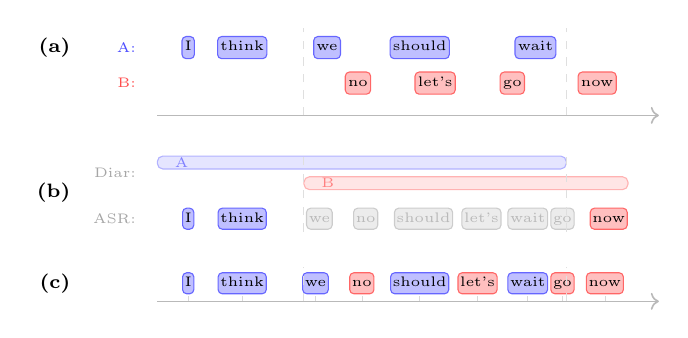
\begin{tikzpicture}[
    xscale=0.98,
    yscale=0.82,
    spkA/.style={fill=blue!25, draw=blue!60, rounded corners=1.5pt, minimum height=0.28cm, inner sep=1pt, font=\tiny\strut},
    spkB/.style={fill=red!25, draw=red!60, rounded corners=1.5pt, minimum height=0.28cm, inner sep=1pt, font=\tiny\strut},
    spkAt/.style={fill=blue!25, draw=blue!60, rounded corners=1.5pt, minimum height=0.26cm, inner sep=0.8pt, font=\tiny\strut},
    spkBt/.style={fill=red!25, draw=red!60, rounded corners=1.5pt, minimum height=0.26cm, inner sep=0.8pt, font=\tiny\strut},
    amb/.style={fill=gray!15, draw=gray!40, rounded corners=1.5pt, minimum height=0.24cm, inner sep=0.8pt, font=\tiny\strut, text=gray!55},
    timeline/.style={->, semithick, gray!55},
    lbl/.style={font=\scriptsize\bfseries, anchor=east},
]

% ---- (a) Ground truth ----
\node[lbl] at (-0.7, 2.6) {(a)};

\node[spkA] at (0.7, 2.6) {I};
\node[spkA] at (1.4, 2.6) {think};
\node[spkA] at (2.5, 2.6) {we};
\node[spkA] at (3.7, 2.6) {should};
\node[spkA] at (5.2, 2.6) {wait};

\node[spkB] at (2.9, 2.05) {no};
\node[spkB] at (3.9, 2.05) {let's};
\node[spkB] at (4.9, 2.05) {go};
\node[spkB] at (6.0, 2.05) {now};

\node[font=\tiny, blue!70, anchor=east] at (0.15, 2.6) {A:};
\node[font=\tiny, red!70, anchor=east] at (0.15, 2.05) {B:};

\draw[timeline] (0.3, 1.55) -- (6.8, 1.55);
\draw[dashed, gray!25, thin] (2.2, 1.55) -- (2.2, 2.9);
\draw[dashed, gray!25, thin] (5.6, 1.55) -- (5.6, 2.9);


% ---- (b) Cascade ----
\node[lbl] at (-0.7, 0.35) {(b)};

\draw[fill=blue!10, draw=blue!30, rounded corners=2pt] (0.3, 0.72) rectangle (5.6, 0.92);
\node[font=\tiny, blue!50, anchor=west] at (0.4, 0.82) {A};
\draw[fill=red!10, draw=red!30, rounded corners=2pt] (2.2, 0.4) rectangle (6.4, 0.6);
\node[font=\tiny, red!50, anchor=west] at (2.3, 0.5) {B};
\node[font=\tiny, gray!70, anchor=east] at (0.15, 0.66) {Diar:};

\node[font=\tiny, gray!70, anchor=east] at (0.15, -0.05) {ASR:};
\node[spkAt] at (0.7, -0.05) {I};
\node[spkAt] at (1.4, -0.05) {think};
\node[amb] at (2.4, -0.05) {we};
\node[amb] at (3.0, -0.05) {no};
\node[amb] at (3.75, -0.05) {should};
\node[amb] at (4.5, -0.05) {let's};
\node[amb] at (5.1, -0.05) {wait};
\node[amb] at (5.55, -0.05) {go};
\node[spkBt] at (6.15, -0.05) {now};

\draw[dashed, gray!25, thin] (2.2, -0.25) -- (2.2, 1.0);
\draw[dashed, gray!25, thin] (5.6, -0.25) -- (5.6, 1.0);


% ---- (c) Shuffle ----
\node[lbl] at (-0.7, -1.05) {(c)};

\node[spkAt] at (0.7, -1.05) {I};
\node[spkAt] at (1.4, -1.05) {think};
\node[spkAt] at (2.35, -1.05) {we};
\node[spkBt] at (2.95, -1.05) {no};
\node[spkAt] at (3.7, -1.05) {should};
\node[spkBt] at (4.45, -1.05) {let's};
\node[spkAt] at (5.1, -1.05) {wait};
\node[spkBt] at (5.55, -1.05) {go};
\node[spkBt] at (6.1, -1.05) {now};

\foreach \x in {0.7, 1.4, 2.35, 2.95, 3.7, 4.45, 5.1, 5.55, 6.1} {
    \draw[gray!30, very thin] (\x, -1.25) -- (\x, -1.33);
}
\draw[timeline] (0.3, -1.33) -- (6.8, -1.33);

\draw[dashed, gray!25, thin] (2.2, -1.33) -- (2.2, -0.8);
\draw[dashed, gray!25, thin] (5.6, -1.33) -- (5.6, -0.8);

\end{tikzpicture}
\caption{%
Word-level speaker attribution in overlapped speech.
\textbf{(a)}~Ground truth: speakers A (\textcolor{blue!60}{blue}) and B (\textcolor{red!60}{red}) produce concurrent tokens with partial overlap (dashed).
\textbf{(b)}~Cascade: diarization detects both speakers as active, but all ASR words in the overlap are ambiguous (gray) since both segments cover the same time.
\textbf{(c)}~Shuffle: the Viterbi path produces an interleaved, time-aligned, speaker-attributed sequence.
}
\label{fig:overlapped_attribution}
\vspace{-4mm}
\end{figure}

In~\cite{wiesner2026modeling} we proposed constructing alignment graphs from the shuffle product of multi-talker transcripts, treating overlapped and non-overlapped speech uniformly and enabling multi-talker forced alignment in a single Viterbi pass. We evaluated the approach on synthetic 30s mixtures of two and three speakers, but it has two limitations addressed here. First, without modification it does not easily scale to longer recordings or more speakers, preventing application to meeting-style speech~\cite{carletta2005ami, vinnikov2024notsofar, cornell2025recent}. Second, it assumes speaker-attributed transcripts, whereas practical transcripts often provide utterance boundaries but no speaker labels. Speaker diarization alone does not resolve this ambiguity in overlapped speech: frame-level activity does not uniquely determine who produced each token.

Assigning utterances to speakers is an instance of the speaker partitioning problem~\cite{brummer2010speaker}, whose solution space grows with the Bell numbers and which clustering methods such as VBx~\cite{landini2022bayesian} solve approximately from acoustics alone. Similar to \cite{9746225},  we instead view diarization as assigning temporally localized labels to speakers. This permits transcript-conditioned diarization, similar in spirit to \cite{shafey19_interspeech, park19_interspeech}: the audio is first aligned to transcripts without speaker labels, after which speaker partitions are scored under the acoustic model given the token alignment.

The contributions of this paper are: (i) inference techniques that make shuffle-based alignment of long recordings with many speakers feasible on a single GPU, evaluated by ablation (Section~\ref{sec:results_longform}); (ii) speaker attribution for transcripts without speaker labels, formulated as token alignment followed by search over speaker partitions using frame-level speaker posteriors from a speaker-attributed shuffle model (Section~\ref{sec:speaker_attribution}); and (iii) out-of-domain evaluation of publicly released models trained only on synthetic and web-scraped data on the AMI and NSF1 single distant microphone (SDM) condition.

%\section{Related Work}
%%The mostly commonly used tool for forced alignment is the Montreal Forced Aligner, which wraps Hybrid HMM/DNN implemented in \textsc{kaldi} into an easy to use python interface. It does not  handle speaker attribution, and generally fails on overlapped speech as will be apparent in Section \ref{sec:experiments}.

%While there has been very little work on multi-talker Viterbi forced alignment apart from our prior work on shuffle models \cite{wiesner2026modeling}, a significant body of work on long-form alignment exists. 

%Recent work \cite{zeyer2026gradient} shows how any ASR system through which we can backpropagate can be repurposed for forced alignment by doing dynamic time warping (DTW) on gradients of the input signal to the system.

%We will have to talk about some systems that must exist for alignment from separation systems. 
%We probably also need to talk about some approaches to long-form alignment.

Forced alignment of single-speaker audio is a well-established problem. HMM-based aligners such as MFA~\cite{mcauliffe2017montreal, povey2011kaldi}, CTC-based aligners~\cite{CTC_align, rastorgueva2023nfa, bain2023whisperx} and recent novel approaches based on saliency~\cite{zeyer2026gradient}, all model one token sequence and one active speaker per frame, and for long recordings they avoid the full Viterbi lattice by segmenting the audio with voice activity detection (VAD) or a first decoding pass and aligning each segment separately~\cite{moreno1998recursive, katsamanis2011sailalign, biased_LMs}. This strategy requires either silent regions at which to segment or a first pass that is accurate enough to provide anchors. The alternative is to keep the exact search and reduce its memory, for instance by checkpointing the Viterbi lattice~\cite{tarnas1998reduced} or by pruning it to a band~\cite{kuang2022pruned}; the techniques of Section~\ref{sec:longform} belong to this second approach.

On the multi-talker side, the situation is reversed: several systems require aligned data but no current single technique can produce it. For example, token-level serialized output training~\cite{kanda2020sot, kanda22_interspeech} is trained on timed, speaker-attributed transcripts, which are currently obtained by aligning the single-speaker source recordings before they are mixed~\cite{polok2026mindgap}. Large-scale data pipelines such as Emilia~\cite{he2024emilia} and Sommelier~\cite{jung2026sommelier} instead apply source separation and diarization to obtain single-speaker segments that a standard aligner can process. This is effective on web audio with limited overlap, but in far-field conversational settings neural speech separation degrades and ceases to be effective, in particular as a front-end for ASR~\cite{cornell2025recent}. Apart from our previous work~\cite{wiesner2026modeling}, we are not aware of prior work on Viterbi forced alignment of overlapped multi-talker transcripts. Moreover, word timing alone is not sufficient for most applications: to be useful, multi-talker alignment must also attribute each word to a speaker. Attributing utterances to speakers without labels is an instance of the speaker partitioning problem of Br\"ummer and de Villiers~\cite{brummer2010partitioning}, whose solution space grows with the Bell numbers and which clustering methods such as VBx~\cite{landini2022vbx} solve approximately. The method of Section~\ref{sec:attribution} differs from both in that it scores speaker partitions of the reference utterances directly under the acoustic model, given a fixed token alignment.
\vspace{-2mm}
\section{Multi-Talker Forced Alignment}
% In this section we formalize the problem of multi-talker alignment and its variations. The fundamental supervision object that we will consider is the \textbf{utterance group} \cite{kanda2021large}, which is simply a collection of transcribed utterances with a reference start and end time associated with an audio input, $\mathbf{x}$. Let $\mathcal{G} = \{u^1, \ldots, u^k\}$, be an utterance group, associated with $\mathbf{x}$. Let $y^i$ be a sequence of tokens describing the audio associated with the utterance, $u^i$, where each token is drawn from vocabulary, $\mathcal{V}$. We assume that for each $u^i \in \mathcal{G}$ we have a single speaker label. Let $\mathcal{S} = \{1, \ldots, s_{max}\}$ be an ordering of up to $s_{max}$ speakers in $\mathbf{x}$, e.g., the order in which speakers first appear, and let $s^i$ be the speaker associated with utterance $u^i$. We consider two scenarios:

% \textbf{Alignment with Speaker Labels} -- The speaker label associated with each utterance is known. The only latent variable is the time alignment. Using speaker labels might improve alignment quality. We will denote speaker attributed versions of variables, with $\prime$, e.g., the speaker attributed token sequence, $y$ would be $y^\prime$.

% \textbf{Alignment without Speaker Labels} -- The speaker label associated with each utterance is an additional latent variable that can be inferred, or marginalized. This task is effectively a form of transcript conditioned diarization, where the transcript, its alignment with the audio, and coarse segment boundaries are used to determine speaker boundaries and attribute words to speakers.

%and let ${y^i}^\prime = (y_1^i, s^i), (y_2^i, s^i), \ldots, (y_N^i, s^i)$ be the speaker attributed token sequence for utterance $u^i$. Let $\mathcal{Y^\prime} = \bigshuffle\limits_{i =1}^k {y^i}^\prime$ be the  shuffle product of the speaker attributed token sequences of utterances in $\mathcal{G}$. Let $a^\prime$ be the \emph{alignment} of ${y^i}^\prime$ to $\mathbf{x}$ obtained by labeling each frame (indexed by $t$) of $\mathbf{x}$ with one of the label from for each frame.
%, speaker pair, $\left(\upsilon_t, \sigma_t\right)$, from $\mathcal{V} \times \mathcal{S}$, or a special no-label symbol, $\oslash$.

% -------------------------------------
We formalize multi-talker alignment and its variations. The fundamental supervision object is the \textbf{utterance group}%~\cite{kanda2021large}
, a collection of transcribed utterances with reference start and end times within
audio input, $\mathbf{x}$. Let $\mathcal{G} = {u^1, \ldots, u^k}$ be an utterance group and $y^i$ the token sequence for utterance $u^i$, with tokens drawn from vocabulary $\mathcal{V}$. Each $u^i \in \mathcal{G}$ has one speaker label. Let $\mathcal{S} = {1, \ldots, s_{\max}}$ denote an ordering of up to $s_{\max}$ speakers in $\mathbf{x}$, e.g., by first appearance, and $s^i$ the speaker associated with $u^i$. We consider two scenarios:

\textbf{Alignment with Speaker Labels} -- The speaker label of each utterance is known and only the time alignment is latent. Speaker labels may improve alignment quality. We denote speaker-attributed variables with $\prime$, e.g., $y^\prime$.

\textbf{Alignment without Speaker Labels} -- The speaker label of each utterance is also latent and can be inferred or marginalized. This is a form of transcript-conditioned diarization, where the transcript, its alignment, and coarse segment boundaries are used to determine speaker boundaries and attribute words to speakers.

Our method involves tackling three subtasks needed for multi-talker forced alignment: (i) alignment algorithms with speaker labels, (ii) fast and memory efficient long-form alignment, and (iii) speaker attribution when the utterance group has no speaker labels.
\vspace{-2mm}
\subsection{Alignment with Speaker Labels Using Shuffles}
\label{sec:SpAShl}
We follow~\cite{wiesner2026modeling}, using the shuffle product of multi-talker transcripts as the alignment graph for single-pass forced alignment, and provide only a high-level summary here. Let ${y^i} = y_1^i, \ldots, y_N^i$ be the token sequence for utterance $u^i \in \mathcal{G}$ and ${y^i}^\prime = (y_1^i,s^i), \ldots, (y_N^i,s^i)$ its speaker-attributed version. Then $\mathcal{Y} = \bigshuffle\limits_{i=1}^k {y^i}$ is the shuffle product and $\mathcal{Y^\prime} = \bigshuffle\limits_{i=1}^k {y^i}^\prime$ its speaker-attributed equivalent. Each element of the shuffle product, equivalently a path through its finite-state automaton (FSA), is an (interleaved) serialization of the tokens from utterances in $\mathcal{G}$. Let $G\left(\mathcal{Y}\right)$ denote the FSA representing $\mathcal{Y}$.


% A CTC-like model can be trained, with the help of a specific CTC topology, $\mathcal{T}$, by marginalizing over both all possible shuffles and over all alignments of shuffles to the audio $\mathbf{x}$. The space of all alignments can be represented as an FSA, $\mathcal{T} \circ G\left(\mathcal{Y}^\prime\right)$. Let $U\left(\mathbf{x}\right)$ be a neural network producing probabilities, $p\left(a_t | \mathbf{x}\right)$, for a frame at time, $t$, over the blank augmented vocabulary, $\oslash \bigcup \mathcal{V}$, or $\oslash \bigcup \left(\mathcal{V} \times \mathcal{S}\right)$ in the speaker attributed case. Then the Viterbi path through \begin{equation} U\left(\mathbf{x}\right) \circ \left(\mathcal{T} \circ G\left(\mathcal{Y}\right)\right)\end{equation} corresponds to the single best interleaving and alignment according to $U\left(\cdot \right)$. Let $a^\prime = a_1^\prime, \ldots, a_T^\prime$ be such an alignment, e.g., \begin{equation} a^\prime = (\_\mbox{hi}, 1), \oslash, (\_\mbox{hey}, 2), \oslash, (\_\mbox{there}, 1).\end{equation}
% In other words,
% \begin{equation}
%     {a^{\prime}}^* = \argmax_{a^\prime \in U\left(\mathbf{x}\right) \circ \left(\mathcal{T} \circ G\left(\mathcal{Y}\right)\right)} p\left(a^\prime | \mathbf{x}\right). \label{eq:alignment}
% \end{equation}

% We will also use the $\beta^{-1}\left(\mathcal{Y}\right)$ as short hand for $\mathcal{T} \circ G\left(\mathcal{Y}\right)$ where the composition with the neural network outputs is implied.

A CTC-like model can be trained with topology $\mathcal{T}$ by marginalizing over all transcript shuffles and their alignments to the audio $\mathbf{x}$. These alignments are represented by the FSA $\mathcal{T}\circ G(\mathcal{Y}^\prime)$. Let $U(\mathbf{x})$ be a neural network producing frame-level probabilities $p(a_t\mid\mathbf{x})$ over the blank-augmented vocabulary ${\oslash}\cup\mathcal{V}$, or ${\oslash}\cup(\mathcal{V}\times\mathcal{S})$ in the speaker-attributed case. The Viterbi path through
\begin{equation}
U(\mathbf{x})\circ\left(\mathcal{T}\circ G(\mathcal{Y}^\prime)\right)
\end{equation}
gives the most likely interleaving and alignment. Let $a^\prime=a_1^\prime,\ldots,a_T^\prime$ denote this alignment, e.g., $a^\prime=(\_\mbox{hi},1),\oslash,(\_\mbox{hey},2),\oslash,(\_\mbox{there},1).$
Thus,
\begin{equation}
{a^\prime}^*=
\argmax_{a^\prime\in U(\mathbf{x})\circ\left(\mathcal{T}\circ G(\mathcal{Y}^\prime)\right)}
p(a^\prime\mid\mathbf{x}).
\label{eq:alignment}
\end{equation}

We also use $\beta^{-1}(\mathcal{Y})$ -- all alignments that map to a serialization in $\mathcal{Y}$ -- as shorthand for $\mathcal{T}\circ G(\mathcal{Y})$, with composition with the neural-network outputs implied.

\subsection{Fast and Efficient Long-form Alignment}
\label{sec:longform_tricks}
Speaker-attributed alignment can in principle be applied directly to real meeting recordings, but these often contain long ($>1$ min) utterance groups without pauses and enough speakers for the shuffle graphs to become very large. Even with the partial-order pruning of~\cite{wiesner2026modeling} and restrictive collars, constructing the full graph can be a bottleneck and consume substantial GPU memory. On the 32\,GiB V100s used for most experiments, naive Viterbi alignment (Section~\ref{sec:SpAShl}) causes out-of-memory errors. We therefore apply three techniques for efficient long-form alignment.


\textbf{1-state CTC-topology} -- We use a 1-state CTC topology~\cite{laptev2022ctc} with a self-loop accepting all symbols, including $\oslash$ instead of the training topology. Since CTC models produce peaky outputs, this has little effect on performance while substantially reducing the topology expansion of the shuffle graph.


\textbf{Blank-frame removal} -- Following~\cite{chen2016phone}, where blank frames are removed prior to constructing transcript lattices to improve efficiency, we remove frames from network outputs, $U\left(\mathbf{x}\right)$, for which $p\left(\oslash \mid \mathbf{x}\right)>\lambda$. The threshold $\lambda$ is tuned on a development set to remove approximately a requested percentage of frames. Storing removed frame indices enables recovering the original timing. Because the shuffle model requires at least as many frames as total transcript tokens, $\oslash$-frames are not pruned in some regions, resulting in a slightly lower effective removal rate than requested.
  

\textbf{Time restricted alignment} -- In long-form data we often have coarse segment timing information, such as start and end times. Similar to time constraints used in \textsc{Kaldi} numerator-graph construction~\cite{povey2016purely}, we apply a token mask that permits only $\oslash$ outside each segment with a collar to account for boundary annotation error.
    
\textbf{Lazy Graph Chunks} -- For very long recordings or spans of heavy multi-speaker overlap, the shuffle graph can become too large to construct. We therefore build the alignment graph in configurable time blocks, similar in spirit to lazy FST construction~\cite{mohri2002weighted} and block Viterbi~\cite{kriouile1990algorithme,BOULIANNE199461}. However, we make no local path decision at block boundaries: all feasible boundary states and their Viterbi scores are retained. Search is exact with respect to the timing constraints. Given the coarse timestamps, we hypothesize a \emph{frontier} of shuffle-graph states at each block boundary. Only frontier states are active at the boundary. Once Viterbi reaches this time, the next graph block is built using the previous frontier as initial states, initialized with their Viterbi scores. The next frontier is estimated assuming uniform token rate between segment start and end times.

In multi-talker alignment, speaker labels defined by start time or total speech duration must be tracked across audio chunks (Figure~\ref{fig:speaker_tracking_ultra_minimal}), used when processing long-form recordings -- it matches training chunks and reduces GPU memory. Because the acoustic model $U\left(\cdot\right)$ assigns speaker-output slots independently for each chunk, the same speaker may receive different labels across chunks. We therefore retain a mapping $\pi_c$ from global speakers to the output slots for chunk $c$. When Viterbi scores are passed across a graph frontier spanning audio chunks, speaker labels are reconciled using $\pi_c$ and $\pi_{c+1}$.

\textbf{BPE Trimming} -- Smaller units can improve alignment by providing finer temporal resolution~\cite{bain2023whisperx}. However, we were unable to train character-level shuffle models because their longer output sequences (length-$N$) greatly increase shuffle-graph size, $\mathcal{O}\left(kN^k\right)$, particularly under heavy overlap ($k$-speakers). At inference, block-wise graph construction makes longer sequences tractable. We therefore recursively decompose BPE units, as in BPE trimming~\cite{sennrich2019revisiting,cognetta-etal-2024-analysis}, but use token length rather than frequency: we choose the shortest decomposition such that no token exceeds a specified length.
% \begin{figure}[htbp]
% \centering
% \begin{tikzpicture}[
%     x=1cm, y=1cm,
%     font=\small,
%     bar/.style={draw, rectangle, rounded corners=2pt, align=center, inner sep=2pt, font=\scriptsize},
%     callout/.style={draw=black!25, fill=black!2, rectangle, rounded corners=2pt, align=center, font=\scriptsize, inner sep=4pt}
% ]

% % Total width budget: ~7.2cm (Fits standard 1-column layout perfectly)

% % =========================================================
% % PART (a): Intra-Audio Chunk Graph Splits
% % =========================================================
% \node[anchor=west, font=\bfseries\small] at (0, 7.8) {(a) Graph Chunks Inside One Audio Chunk};

% % 30s Audio Input Context
% \node[bar, fill=inputbg, draw=inputborder, minimum width=7.2cm, minimum height=0.45cm] at (3.6, 7.2) {
%     \textbf{Audio Input $c$} \textit{(15s -- 45s)}
% };

% % 20s Retained Center
% \node[bar, fill=retainedbg, draw=retainedborder, minimum width=4.8cm, minimum height=0.45cm] at (3.6, 6.55) {
%     \textbf{Retained Output Center $c$} \textit{(20s -- 40s)}
% };

% % 2x 10s Graph Chunks
% \node[bar, fill=graphbg1, draw=graphborder1, minimum width=2.3cm, minimum height=0.45cm] at (2.35, 5.9) {
%     [20--30s] \textbf{($\pi_c$)}
% };
% \node[bar, fill=graphbg1, draw=graphborder1, minimum width=2.3cm, minimum height=0.45cm] at (4.85, 5.9) {
%     [30--40s] \textbf{($\pi_c$)}
% };

% \node[font=\scriptsize, color=black!70] at (3.6, 5.35) {
%     \textit{All graph sub-chunks share the identical speaker map $\pi_c$.}
% };

% % Separator line
% \draw[black!20, thick] (0, 5.0) -- (7.2, 5.0);

% % =========================================================
% % PART (b): Inter-Audio Chunk Graph Splits
% % =========================================================
% \node[anchor=west, font=\bfseries\small] at (0, 4.6) {(b) Graph Chunks Across Audio Chunks};

% % Overlapping Audio Context Inputs
% \node[bar, fill=inputbg!70, draw=inputborder!70, minimum width=4.2cm, minimum height=0.4cm] at (2.1, 4.0) {
%     Audio Input $c$ \textit{[-5s -- 25s]}
% };
% \node[bar, fill=inputbg!70, draw=inputborder!70, minimum width=4.2cm, minimum height=0.4cm] at (5.1, 3.45) {
%     Audio Input $c+1$ \textit{[15s -- 45s]}
% };

% % Non-overlapping Contiguous Retained Centers
% \node[bar, fill=retainedbg, draw=retainedborder, minimum width=3.4cm, minimum height=0.45cm] at (1.7, 2.8) {
%     Retained $c$ \textit{[0s -- 20s]}
% };
% \node[bar, fill=retainedbg, draw=retainedborder, minimum width=3.4cm, minimum height=0.45cm] at (5.3, 2.8) {
%     Retained $c+1$ \textit{[20s -- 40s]}
% };

% % Graph Chunks laid out directly under their respective centers
% \node[bar, fill=graphbg1, draw=graphborder1, minimum width=1.6cm, minimum height=0.45cm] at (0.8, 2.15) {
%     [0--10s] \textbf{$\pi_c$}
% };
% \node[bar, fill=graphbg1, draw=graphborder1, minimum width=1.6cm, minimum height=0.45cm] at (2.6, 2.15) {
%     [10--20s] \textbf{$\pi_c$}
% };

% \node[bar, fill=graphbg2, draw=graphborder2, minimum width=1.6cm, minimum height=0.45cm] at (4.4, 2.15) {
%     [20--30s] \textbf{$\pi_{c+1}$}
% };
% \node[bar, fill=graphbg2, draw=graphborder2, minimum width=1.6cm, minimum height=0.45cm] at (6.2, 2.15) {
%     [30--40s] \textbf{$\pi_{c+1}$}
% };

% % Mapping Transition Box
% \node[callout, minimum width=7.2cm] at (3.6, 1.0) {
%     \textbf{Speaker Mapping Transition Across Audio Boundary:}\\
%     \textbf{Chunk $c$ ($\pi_c$):} Alice $\to$ Slot 0, Bob $\to$ Slot 1\\
%     \textbf{Chunk $c+1$ ($\pi_{c+1}$):} Alice $\to$ \textbf{Slot 1}, Bob $\to$ \textbf{Slot 0}\\
%     \vspace{1pt}
%     \textit{Retained graph chunks step cleanly from $\pi_c$ to $\pi_{c+1}$ at 20s.}
% };

% \end{tikzpicture}
% \caption{Structural breakdown showing how Viterbi graph chunks inherit speaker maps within a single audio chunk (a) versus across contiguous audio chunk boundaries (b).}
% \label{fig:speaker_tracking_parallel}
% \end{figure}


\begin{figure}[htbp]
\centering
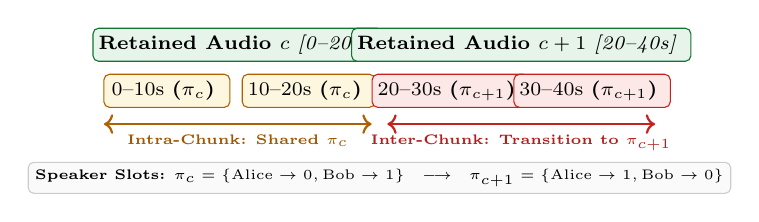
\begin{tikzpicture}[
    x=1cm, y=0.65cm,
    font=\small,
    bar/.style={draw, rectangle, rounded corners=2pt, align=center, inner sep=2pt, font=\scriptsize}
]

% Total width: 7.0cm (Fits 1-column IEEE/ACL layout)

% 1. Contiguous Retained Audio Output Centers
\node[bar, fill=retainedbg, draw=retainedborder, minimum width=3.4cm, minimum height=0.42cm] at (1.7, 2.5) {
    \textbf{Retained Audio $c$} \textit{[0--20s]}
};
\node[bar, fill=retainedbg, draw=retainedborder, minimum width=3.4cm, minimum height=0.42cm] at (5.3, 2.5) {
    \textbf{Retained Audio $c+1$} \textit{[20--40s]}
};

% 2. Graph Sub-Chunks
% Inside Chunk c (Intra-chunk: Both use \pi_c)
\node[bar, fill=graphbg1, draw=graphborder1, minimum width=1.6cm, minimum height=0.42cm] at (0.8, 1.6) {
    0--10s \textbf{($\pi_c$)}
};
\node[bar, fill=graphbg1, draw=graphborder1, minimum width=1.6cm, minimum height=0.42cm] at (2.6, 1.6) {
    10--20s \textbf{($\pi_c$)}
};

% Inside Chunk c+1 (Inter-chunk boundary at 20s -> switches to \pi_{c+1})
\node[bar, fill=graphbg2, draw=graphborder2, minimum width=1.6cm, minimum height=0.42cm] at (4.4, 1.6) {
    20--30s \textbf{($\pi_{c+1}$)}
};
\node[bar, fill=graphbg2, draw=graphborder2, minimum width=1.6cm, minimum height=0.42cm] at (6.2, 1.6) {
    30--40s \textbf{($\pi_{c+1}$)}
};

% 3. Minimal Annotations
\draw[thick, graphborder1, <->] (0.0, 0.95) -- (3.4, 0.95) 
    node[midway, below, font=\tiny\bfseries, color=graphborder1!90!black] {Intra-Chunk: Shared $\pi_c$};

\draw[thick, graphborder2, <->] (3.6, 0.95) -- (7.0, 0.95) 
    node[midway, below, font=\tiny\bfseries, color=graphborder2!90!black] {Inter-Chunk: Transition to $\pi_{c+1}$};

% 4. One-Line Permutation Legend
\node[draw=black!20, fill=black!2, rectangle, rounded corners=2pt, font=\tiny, inner sep=2.5pt] at (3.5, -0.1) {
    \textbf{Speaker Slots:} $\pi_c = \{\text{Alice}\to0, \text{Bob}\to1\} \;\;\longrightarrow\;\; \pi_{c+1} = \{\text{Alice}\to1, \text{Bob}\to0\}$
};

\end{tikzpicture}
\caption{Unified speaker mapping mechanism: sub-chunks within audio chunk $c$ inherit $\pi_c$, while crossing the 20s boundary transitions directly to $\pi_{c+1}$.}
\label{fig:speaker_tracking_ultra_minimal}
\end{figure}

\vspace{-5mm}
\subsection{Alignment without Speaker Labels}
\label{sec:speaker_attribution}
Our aim is to jointly align and attribute tokens to speakers. Section~\ref{sec:SpAShl} considered this problem when utterance speaker labels are known. Without speaker labels, we decompose it into two steps: (i) find the best token alignment over the speaker-independent shuffle product $\mathcal{Y}$; and (ii) find the best partition of utterances among speakers given this alignment.

% Let $\mathcal{P}=\{\mathcal{P}_{1},\ldots,\mathcal{P}_{m}\}$ be a partition of the $k$ utterances in $\mathcal{G}$ into $m\leq s_{\max}\leq k$ speakers, where $s_{\max}=k$ if the number of speakers is unconstrained. Let $g(u^i,\mathcal{P})=j$ if $u^i\in\mathcal{P}_{j}$, and let $\mathbf{P}$ denote the set of feasible partitions. Since a speaker-attributed alignment can be defined by a token alignment and a partition,
% \begin{align}
% {a^\prime}^*
% &=\argmax_{a\in\beta^{-1}(\mathcal{Y}),\,\mathcal{P}\in\mathbf{P}}
% p(a\mid\mathbf{x})p(\mathcal{P}\mid a,\mathbf{x}).
% \end{align}
% We approximately solve this joint optimization by
% \begin{align}
% a^* &= \argmax_{a\in\beta^{-1}(\mathcal{Y})}p(a\mid\mathbf{x}),\\
% \mathcal{P}^* &= \argmax_{\mathcal{P}\in\mathbf{P}}
% p(\mathcal{P}\mid\mathbf{x},a^*).
% \end{align}

% Although speaker labels are unknown, utterance indices can be retained on tokens during alignment while using only $p(\upsilon_t\mid\mathbf{x})$ for the arc weights. Thus $a^*$ identifies the non-$\oslash$ frames aligned to each utterance. Let
% \begin{equation}
% \mathcal{T}_{u^i}
% =
% \{t\mid a_t^*=(\upsilon,i),\,\upsilon\neq\oslash\}.
% \end{equation}

% For the factored joint shuffle model~\cite{wiesner2026modeling}, only non-blank frames contribute to the probability of a partition. Let $\bar{\oslash}$ denote the event that the token emitted at a frame is nonblank. We then write
% \begin{align}
% p(\mathcal{P}\mid\mathbf{x},a^*)
% &=\prod_{i=1}^{k}\prod_{t\in\mathcal{T}_{u^i}}
% p_{\sigma_t}\left(g(u^i,\mathcal{P})\mid\mathbf{x},\bar{\oslash}\right)\\
% &=\prod_{i=1}^{k}G(\mathcal{P},u^i),
% \end{align}
% and therefore
% \begin{equation}
% \mathcal{P}^*=
% \argmax_{\mathcal{P}\in\mathbf{P}}
% \prod_{i=1}^{k}G(\mathcal{P},u^i).
% \end{equation}

Let $\mathcal{P}=\{\mathcal{P}_{1},\ldots,\mathcal{P}_{m}\}$ be a partition
of the $k$ utterances in $\mathcal{G}$ into $m\leq s_{\max}\leq k$ speakers,
where $s_{\max}=k$ if unconstrained. Let $g(u^i,\mathcal{P})=j$ if
$u^i\in\mathcal{P}_{j}$, and let $\mathbf{P}$ denote the set of feasible
partitions. Since a speaker-attributed alignment can be defined by a token
alignment and a partition,
\begin{equation}
{a^\prime}^*
=
\argmax_{\substack{a\in\beta^{-1}(\mathcal{Y})\\
                   \mathcal{P}\in\mathbf{P}}}
p(a\mid\mathbf{x})p(\mathcal{P}\mid a,\mathbf{x}).
\end{equation}
We approximately solve this joint optimization by
\begin{equation}
\begin{gathered}
a^*
=
\argmax_{a\in\beta^{-1}(\mathcal{Y})}
p(a\mid\mathbf{x}),\\
\mathcal{P}^*
=
\argmax_{\mathcal{P}\in\mathbf{P}}
p(\mathcal{P}\mid\mathbf{x},a^*).
\end{gathered}
\end{equation}

Although speaker labels are unknown, utterance indices can be retained on
tokens during alignment while using only $p(\upsilon_t\mid\mathbf{x})$ for
the arc weights. Thus $a^*$ identifies the non-$\oslash$ frames aligned to
each utterance; let
$\mathcal{T}_{u^i}=\{t\mid a_t^*=(\upsilon,i),\,\upsilon\neq\oslash\}$.

For the factored joint shuffle model~\cite{wiesner2026modeling}, only
non-blank frames contribute to the probability of a partition. Let
$\bar{\oslash}$ denote the event that the token emitted at a frame is
nonblank. We then write
\begin{equation}
\begin{gathered}
p(\mathcal{P}\mid\mathbf{x},a^*)
=
\prod_{i=1}^{k}\prod_{t\in\mathcal{T}_{u^i}}
p_{\sigma_t}\!\left(
g(u^i,\mathcal{P})\mid\mathbf{x},\bar{\oslash}
\right)
=
\prod_{i=1}^{k}G(\mathcal{P},u^i),\\
\mathcal{P}^*
=
\argmax_{\mathcal{P}\in\mathbf{P}}
\prod_{i=1}^{k}G(\mathcal{P},u^i).
\end{gathered}
\end{equation}

For a few utterances, $\mathcal{P}^*$ can be found by brute force search over $\mathbf{P}$. We instead greedily assign each utterance to the element of the partition (speaker) that maximizes $G\left(\mathcal{P}, u^i\right)$.













% --------------------------------------
% Our aim is to jointly align and attribute token sequences to speaker. In Section \ref{sec:SpAShl} we saw how to solve this problem when utterances were labeled with speaker. 

% Consider the shuffle product obtained from only the token sequences, i.e., not considering speaker, and denote this as $\mathcal{Y}$. If speaker labels are not present, we propose to decompose this problem into two steps: (i) find the best token alignment without considering speaker labels, i.e., finding the best path among $\beta^{-1}\left(\mathcal{Y}\right)$; (ii) find the best partition of segments among speakers given the alignment. Let $\mathcal{P} = \{\mathcal{P}_{s_1}, \ldots, \mathcal{P}_{s_{max}}\}$ be a partition of the $k$ utterances in $\mathcal{G}$, into at most $k$ speakers, let $g: \left(u^i, \mathcal{P}\right) \to s \ \ s.t.  \ \ u^i \in \mathcal{P}_s$ be the map from an utterance, $u^i$ to its index in partition $\mathcal{P}$, and let $\mathbf{P}$ be a set of feasible partitions, for instance, all Partitions into at most $s_{max}$ speakers. Note that a speaker attributed alignment can be equivalently defined by a token alignment and a partition. Formally, the problem can be stated as,
% \begin{align}
%     {a^\prime}^* &= \left(a^*, \mathcal{P}^*\right)\\
%    &= \argmax_{a \in \beta^{-1}\left(\mathcal{Y}\right), \mathcal{P} \in \mathbf{P}} p\left(a, \mathcal{P} | \mathbf{x}\right) \\
%    &= \argmax_{a \in \beta^{-1}\left(\mathcal{Y}\right), \mathcal{P} \in \mathbf{P}} p\left(a | \mathbf{x}\right) p\left(\mathcal{P} | a, \mathbf{x}\right).
% \end{align}
% We propose to approximately solve the attributed alignment problem by 
% \begin{align}
%      a^* &= \argmax_{a\in \beta^{-1}\left(\mathcal{Y}\right)} p\left(a | \mathbf{x}\right) \\
%      \mathcal{P}^* &= \argmax_{\mathcal{P} \in \mathbf{P}} p\left(\mathcal{P} | \mathbf{x}, a^*\right).
% \end{align}

% % Brümmer et. al \cite{brummer2010speaker} and van Leeuwen \cite{leeuwen2010speaker}, discuss the task of speaker partitioning, the combinatorial search space inherent to this task, and consequently to speaker diarization. 
% %For this reason both mostly discarded direct search over speaker partitions in favor of clustering based approximations that are more scalable with the number of utterances. However, 
% % Different from clustering-based approaches to solve the partitioning problem, directly search over the space of all speaker partitions may be possible when the number of utterances is small enough, such as within utterance groups.

% % Let $\mathcal{Y}_\mathcal{P}^\prime$ be the speaker augmented shuffle graph for a speaker partition, $\mathcal{P}$, recalling that it is equivalent to $\mathcal{Y}$ with some additional speaker tags on arcs. Let $ \mathcal{Y}^{\prime\prime} = \bigcup_\mathcal{P} \mathcal{\mathcal{Y}_{\mathcal{P}}^\prime}$
% % be the union of all shuffle products assuming different speaker partitions. This graph encodes all valid ways of interleaving $u_y^1, \ldots, u_y^k$ for all speaker partitions.

% % This set is very large: the number of possible speaker partitions is given by the Bell number \cite{bell1938iterated, becker1948arithmetic}, $B_k = (1, 2, 5, 15, 52, 203, ...)_k$, so $\mathcal{Y}^{\prime\prime}$ will be that many times as big as the already large shuffle, $\mathcal{Y}$. Running even a pruned Viterbi algorithm on this graph is expensive. However, reducing this problem to comparing possible speaker partitions for a single alignment, makes the problem tractable for the vast majority of utterance groups ($B_9 = 21147$).
% % Limiting the maximum number of possible speakers to $s_{max}$ reduces the number of partitions to $\sum_{i=1}^{s_{max}} S\left(k, s\right)$, where $S\left(k, s\right)$ is the Stirling number of the second kind~\cite{}, which grows more slowly with $k$.

% Although we do not know the speaker labels, we do not need to discard the utterance indices associated with each token during alignment. We can include them in place of the speaker tags, and use only $p\left(\upsilon_t | \mathbf{x}\right)$ for the arc weights. Then the optimal alignment, $a^*$, will include utterance indices on the non-$\oslash$ output frames. Let $\mathcal{T}_{u^i} = \{ t \mid a_t^* = (\bar{\oslash},i) \}$ be the set of non-blank tokens that aligned to each utterance $u^i$.

% Note that in the factored joint shuffle model \cite{wiesner2026modeling}, given an alignment, the only frames that contribute to the probability of a particular partition are the non-blank frames. We model the probability of a partition as

% \begin{align}
%     p\left(\mathcal{P} | \mathbf{x}, a^*\right)
%     &= \prod_{i=1}^{k} \prod_{t\in \mathcal{T}_{u^i}} p_{\sigma_t}\left(g\left(u^i, \mathcal{P}\right) | \ \mathbf{x}, \bar{\oslash}\right) \\
%     &= \prod_{i=1}^k G\left(\mathcal{P}, u^i\right),
% \end{align}
% and therefore,
% \begin{equation}
%     \argmax_{\mathcal{P} \in \mathbf{P}} p\left(\mathcal{P} | \mathbf{x}, a^*\right) 
%     = \argmax_{\mathcal{P} \in \mathbf{P}} \prod_{i=1}^k G\left(\mathcal{P}, u^i\right).
% \end{equation}

% If the number of partitions, or equivalently utterances, is relatively small, we could search exhaustively over all partitions. We propose a simple method, which is to consider each utterance independently. Actually, this search method is exact if the set of feasible partitions is unconstrained. 
% %However, using speaker labels that have some semantic meaning, such as speaker appearance order, or rank by amount of speech, constrains the set of feasible partitions, $\mathbf{P}$, and independent assignment is no longer exact. Therefore, our other approach is to represent the set of feasible partitions as a graph with paths, all of length $k$, representing speaker assignments for each of the $k$ utterances. A partition is just one path in this graph, and it can also be found via beam search.

% %This procedure also provides a diagnostic for the quality of the speaker labeling for speaker attributed ASR systems. Completely disentangling the effects of speaker attribution from token recognition is difficult; performance is normally measured wholistically using metrics such as cpWER \cite{}. Some LLM-based post-processing proposed using word diarization error rate (WDER) since their systems are label synchronous and cannot be used to evaluate frame-level DER. However, the metric is somewhat flawed because the metric not take into account insertions or deletions, and tokens are attributed after recognition, which may be errorful. The procedure described above can be used to completely disentangle attribution from token recognition and measure speaker attribution given the single best alignment of the ground-truth transcripts.


% % Now if the term $G\left(\mathcal{P}, u^i\right)$, can be optimized sequentially, or even, independently for each utterance, $u^i$, then we can separate the assignment problem by sequentially picking the best scoring speaker given the remaining valid partitions.
% % % \begin{equation}
% % %     \max_{\mathcal{P} \in \mathbf{P}} \prod_{i=1}^k G\left(\mathcal{P}, u^i\right) = \prod_{i=1}^k \max_{\mathcal{P}_{s} | \mathcal{P} \in \mathbf{P}} G\left(\mathcal{P}_s, u^i \right).
% % % \end{equation}
% % If speakers are labeled according to start time, then the partitions are constrained to be restricted growth strings \cite{silnova2020probabilistic}, \begin{equation}
% %     \mathcal{R} = \{r | r_n \leq \max_{m < n} r_m + 1\}.
% % \end{equation}
% % These are strings such as $\{00, 01, 012, 010, 0102\}$, where the value of the next symbol can be at most one more than the maximum among the previous symbols. Each growth string can be mapped via $F^{-1}: r \to \mathcal{P}$, from a string $r \in \mathcal{R}$ to a partition, $\mathcal{P}$. Then the optimal partition,
% % \begin{equation}
% %     \mathcal{P}^* = \argmax_{r \in \mathcal{R}} \prod_{i=1}^k G\left(F^{-1}\left(r\right), u^i\right).
% % \end{equation}

% % We can do a prefix search over these strings with a beam to approximately find the optimal partition. In the case of greedy search, $\mathcal{P}^*$ can be found recursively as,
% % \begin{align}
% %     r_i^* &= \argmax_{s_i} \ \prod\limits_{t \in \mathcal{T}_{u^i}}p_{\sigma_t}\left(s_i | \mathbf{x}, \bar{\oslash}\right), \\
% %     \mbox{ and } \mathcal{P}^* &= F\left(r_1^*\cdots r_k^*\right).
% % \end{align}

% % \textbf{Diarization via Joint Alignment} -- We can extend the alignment algorithm in Equation \ref{eq:alignment} to work when the speaker labels are unknown by augmenting the shuffle graph to include all possible speaker assignments of the shuffled utterances. Let $\mathbf{s} \in \mathcal{S}^k$ be a speaker assignment vector for the utterances in $\mathcal{G}$, and $\mathcal{Y}_\mathbf{s}^\prime$ be the speaker augmented shuffle graph for a speaker assignment, $\mathbf{s}$. Finally, let
% % \begin{equation}
% %     \mathcal{Y}^{\prime\prime} = \bigcup\limits_{\mathbf{s}} \mathcal{\mathcal{Y}_{\mathbf{s}}^\prime}
% % \end{equation}
% % be the union of all shuffle products assuming different speaker assignments. The optimal alignment $a^* =(\upsilon, \sigma)$ corresponds to the arc labels on the Viterbi path through the supervision graph, $G\left(\mathcal{Y}^{\prime\prime}\right)$. The size of this graph is prohibitively large --- for $k$ utterances the number of possible speaker assignments is the number of possible utterance partitions, also known as the Bell number \cite{bell1938iterated, becker1948arithmetic}, $B_k= \left(1, 2, 5, 15, 52, 203, \ldots \right)_k$ -- so it will be that many times as big as the already large shuffle graph, $\mathcal{Y}$. For anything beyond $k=3$, this approach requires lazy construction of the graph to avoid storing it all in memory and exhaustively exploring all paths. 

% % \textbf{Diarization by Marginalizing over Alignments} -- Instead of finding the speaker assignment and token alignment that is \emph{jointly} most probable, we could instead first find the \emph{marginally} most likely speaker assignment over all possible token serializations, and then use that for alignment. Instead of running the Viterbi algorithm a single time through a large graph, $G\left(\bigcup_{\mathbf{s}} \mathcal{Y}_\mathbf{s}^\prime\right)$, we compute the Viterbi path using the supervision graph corresponding to the optimal speaker assignment, $G\left(\mathcal{Y}_{\mathbf{s}^*}^\prime\right)$. However, finding the optimal assignment requires running the forward algorithm on \emph{all possible} supervision graphs, $G\left(\mathcal{Y}_\mathbf{s}^\prime\right)$, and then picking the assignment that resulted in the maximum likelihood. Formally,
% % \begin{align}
% %     \mathbf{s}^* &= \argmax\limits_{\mathbf{s}} p\left(\mathcal{G}_\mathbf{s} | \mathbf{x}, \mathbf{s}\right), \\
% %     a^* &= \argmax\limits_{a \in \beta^{-1}\left(\mathcal{Y}_{\mathbf{s}^*}^\prime\right)} p\left(a | \mathbf{x}\right).
% % \end{align}

% % One advantage of this approach is that we do not require $\mathcal{Y}^{\prime\prime}$, so the graphs, $G\left(\mathcal{Y}_{\mathbf{s}}^\prime\right)$, can be constructed sequentially, which mitigates the memory footprint of the algorithm. However, this also means that for $k$ utterances, the forward algorithm must be run for $B_k$ times. For up to $k=5$, this might be possible, but it is extremely slow and anything beyond $k=3$ utterances is not practical. This is the most computationally expensive approach.

% % \textbf{Alignment Conditioned Diarization} -- This last method is the most computationally tractable and is what we actually implemented. If the optimal interleaved sequence of tokens was known, then we could find the \emph{conditionally} most likely speaker assignments considering only a single element $y \in \mathcal{Y}$.

% % One important point -- even though we do not know the speaker labels, we do not need to discard the utterance indices associated with each token during alignment. In fact, these can be included as an (additional) output label on the shuffle graph, or as a tuple where the speaker label is replaced with an utterance index. However, the arc weights come only from $p\left(\upsilon_t | \mathbf{x}\right)$. Let $\omega^*$, be the optimal frame-level utterance tags resulting from the token-level alignment, such that $a^* = \left(\upsilon^*, \omega^*\right)$. Let, $\tau_i = \{t\ |\ \omega_t^* = i\}$ be the set of frames that belong to the $i^{th}$ utterance. Note that because we are assuming single speaker utterances, and we \emph{do} have access to the utterance indices, a speaker assignment will induce a corresponding sequence of speakers for an associated interleaved token sequence. In other words, given the token / segment alignment for $k$ utterances, the frame-level speaker tags, $\sigma$, are a function of $\mathbf{s}$, i.e., $\sigma: \left((\tau)_k, \mathbf{s}\right) \to \sigma$.
% % Each possible speaker assignment is then compared. 

% % Let $a_\mathbf{s}^*$ be the sequence of tuples created from the best token alignment, $\upsilon^*$, and the induced speaker labels when using speaker assignment, $\mathbf{s}$, and let $y_\mathbf{s}^* = \beta\left(a_{\mathbf{s}}^*\right)$, i.e., with the $\oslash$ symbols removed. We could, for instance, construct the graph, $G\left(\bigcup_{\mathbf{s}}y_\mathbf{s}^*\right)$, for each possible speaker assignment, and find this optimal alignment via:

% % \begin{align}
% %     y^* &= \beta\left(\argmax\limits_{a \in \beta^{-1}\left(\mathcal{Y}\right)} p\left(a | \mathbf{x}\right)\right) \\
% %     a^* &= \argmax\limits_{a \in \beta^{-1}\left(\bigcup_\mathbf{s} y_\mathbf{s}^*\right)} p\left(a | \mathbf{x}\right).
% % \end{align}

% % However, we can significantly simplify the search over speaker assignments. Consider the score along a single path where we have assumed, as in CTC, that the alignments at different times given the input $\mathbf{x}$ are conditionally independent, i.e.,
% % \begin{equation}
% %     p\left(a | \mathbf{X}\right) = \prod_{t=1}^T p\left(\upsilon_t | \mathbf{x}\right)p\left(\sigma_t | \upsilon_t, \mathbf{x}\right).
% % \end{equation}

% % The best scoring speaker assignment, $\mathbf{s}^*$, is given by the following optimization:
% % \begin{align}
% %     &\max\limits_{\mathbf{s}} \prod_{t=1}^T p\left(\upsilon_t^* | \mathbf{x}\right)p\left(\sigma_t\left(\mathbf{s}\right) | \upsilon_t^*, \mathbf{x}\right) \\
% %     &= \prod_{t=1}^T p\left(\upsilon_t^* | \mathbf{x}\right)\max\limits_{\mathbf{s}} \prod_{t=1}^T p\left(\sigma_t\left(\mathbf{s}\right) | \upsilon_t, \mathbf{x}\right) \\
% %     &= \prod_{t=1}^T p\left(\upsilon_t^* | \mathbf{x}\right) \max\limits_{\mathbf{s}} \prod_{i=1}^k \prod_{t \in \tau_i} p\left(\mathbf{s}_i | \upsilon_t, \mathbf{x}\right) \\
% %     &=  \prod_{t=1}^T p\left(\upsilon_t^* | \mathbf{x}\right) \prod_{i=1}^k\max\limits_{\mathbf{s}_i} \prod_{t \in \tau_i} p\left(\mathbf{s}_i| \upsilon_t, \mathbf{x}\right) \label{eq:prefix}
% % \end{align}

% % Since the maximum is the product of $k$ independent values, we see that the speaker assignment can be optimized \emph{locally} per segment as long as the joint probability of $p\left(a_t | \mathbf{x}\right) = p\left(\upsilon_t  |\mathbf{x}\right) p\left(\sigma_t | \upsilon_t, \mathbf{x}\right)$. 
% % Therefore, we can use the factored joint model described in Section
% % \ref{sec:speaker_attribution}, to significantly reduce the search.
\section{Experiments}
% \begin{table*}[htbp]
% \centering
% \caption{Baseline Comparison Across Short-form Datasets}
% \label{tab:baselines}
% \begin{tabular}{l ccc ccc ccc}
% \toprule
% & \multicolumn{3}{c}{\textbf{dev3spk}} & \multicolumn{3}{c}{\textbf{NOTSOFAR dev}} & \multicolumn{3}{c}{\textbf{NOTSOFAR eval}} \\
% \cmidrule(lr){2-4} \cmidrule(lr){5-7} \cmidrule(lr){8-10}
% \textbf{Baselines} & \textbf{IoU} $\uparrow$ & \textbf{BE} $\downarrow$ & $\tau$ \% $\downarrow$& \textbf{IoU} $\uparrow$& \textbf{BE} $\downarrow$ & $\tau$ \% $\downarrow$& \textbf{IoU} $\uparrow$ & \textbf{BE} $\downarrow$ & $\tau$ \% $\downarrow$ \\
% \midrule
% Uniform interpolation  (Audio free) & 15.9 & 375 & 77.4 & 38.0 & 170 & 11.2 & 39.8 & 185 & 17.9 \\
% MFA \cite{}& 38.2 & 332 & 113.1 & 50.2 & 307 & 38.8 & 45.8 & 330 & 73.5 \\
% Wav2Vec2 CTC \cite{} & 49.8 & 251 & 91.6 & 51.0 & 240 & 32.4 & 48.4 & 258 & 59.8 \\
% \midrule
% CTC graph per supervision & 59.8 & 73 & 14.2 & 56.3 & 133 & 14.3 & 56.4 & 131 & 26.0 \\
% Orig Paper & 58.2 & 81 & 16.9 & -- & -- & -- & -- & -- & -- \\
% WavLM (reproduction) & 59.0 & 77 & 16.6 & -- & -- & -- & -- & -- & -- \\
% \midrule
% \textbf{New Models} \\
% \midrule
% WavLM 8spk (72k) & 59.9	& 72 & 13.0 & 58.3 & 115 & 9.3 & 58.6	& 104 & 17.4 \\
% WavLM 8spk (72k) (token only) & 59.7 & 73 & 13.0 & 57.8 & 123	& 10.6 & 58.0 & 116	& 19.1 \\
% WAVLM 8spk (72k) + BPE decomposition	& 64.1 & 63 & 12.8 & 60.9	& 105 &	9.0	&	61.3 & 96 & 17.5 \\
% \midrule
% \textbf{Long-form Tricks} \\
% \midrule
% WavLM 8spk (72k) + 1-state topo & 60.1 & 71 & 12.7 & 58.4 & 113 & 9.1 & 58.6 & 102 & 17.2 \\
% \quad + 30\% frames & 60.1 & 71 & 12.7 & 57.0 & 121 & 9.6 & 57.5 & 109 & 17.4 \\
% \quad + 10s graph chunks & 60.1 & 71 & 12.7 & 57.6 & 117 & 9.4 & 57.9 & 105 & 17.3 \\
% \bottomrule
% \end{tabular}
% \end{table*}

% -------------------------------

% \begin{table*}[htbp]
% \centering
% \caption{Baseline Comparison Across Short-form Datasets (Color-Coded by Performance Tier)}
% \label{tab:baselines_colored}
% \begin{tabular}{l ccc ccc ccc}
% \toprule
% & \multicolumn{3}{c}{\textbf{dev3spk}} & \multicolumn{3}{c}{\textbf{NOTSOFAR dev}} & \multicolumn{3}{c}{\textbf{NOTSOFAR eval}} \\
% \cmidrule(lr){2-4} \cmidrule(lr){5-7} \cmidrule(lr){8-10}
% \textbf{Baselines} & \textbf{IoU} $\uparrow$ & \textbf{BE} $\downarrow$ & $\tau$ \% $\downarrow$& \textbf{IoU} $\uparrow$& \textbf{BE} $\downarrow$ & $\tau$ \% $\downarrow$& \textbf{IoU} $\uparrow$ & \textbf{BE} $\downarrow$ & $\tau$ \% $\downarrow$ \\
% \midrule
% Uniform interpolation (Audio free) & \cellcolor{negpoor}15.9 & \cellcolor{negpoor}375 & \cellcolor{negpoor}77.4 & \cellcolor{negpoor}38.0 & \cellcolor{negpoor}170 & \cellcolor{negpoor}11.2 & \cellcolor{negpoor}39.8 & \cellcolor{negpoor}185 & \cellcolor{negpoor}17.9 \\
% MFA \cite{} & \cellcolor{negpoor}38.2 & \cellcolor{negpoor}332 & \cellcolor{negpoor}113.1 & \cellcolor{negpoor}50.2 & \cellcolor{negpoor}307 & \cellcolor{negpoor}38.8 & \cellcolor{negpoor}45.8 & \cellcolor{negpoor}330 & \cellcolor{negpoor}73.5 \\
% Wav2Vec2 CTC \cite{} & \cellcolor{negpoor}49.8 & \cellcolor{negpoor}251 & \cellcolor{negpoor}91.6 & \cellcolor{negpoor}51.0 & \cellcolor{negpoor}240 & \cellcolor{negpoor}32.4 & \cellcolor{negpoor}48.4 & \cellcolor{negpoor}258 & \cellcolor{negpoor}59.8 \\
% \midrule
% CTC graph per supervision & \cellcolor{neutral}59.8 & \cellcolor{neutral}73 & \cellcolor{neutral}14.2 & \cellcolor{neutral}56.3 & \cellcolor{neutral}133 & \cellcolor{neutral}14.3 & \cellcolor{neutral}56.4 & \cellcolor{neutral}131 & \cellcolor{neutral}26.0 \\
% Orig Paper & \cellcolor{neutral}58.2 & \cellcolor{neutral}81 & \cellcolor{neutral}16.9 & -- & -- & -- & -- & -- & -- \\
% WavLM (reproduction) & \cellcolor{neutral}59.0 & \cellcolor{neutral}77 & \cellcolor{neutral}16.6 & -- & -- & -- & -- & -- & -- \\
% \midrule
% \textbf{New Models} \\
% \midrule
% WavLM 8spk (72k) & \cellcolor{posgood}59.9 & \cellcolor{posgood}72 & \cellcolor{posgood}13.0 & \cellcolor{posgood}58.3 & \cellcolor{posgood}115 & \cellcolor{posgood}9.3 & \cellcolor{posgood}58.6 & \cellcolor{posgood}104 & \cellcolor{posgood}17.4 \\
% WavLM 8spk (72k) (token only) & \cellcolor{posgood}59.7 & \cellcolor{posgood}73 & \cellcolor{posgood}13.0 & \cellcolor{posgood}57.8 & \cellcolor{posgood}123 & \cellcolor{posgood}10.6 & \cellcolor{posgood}58.0 & \cellcolor{posgood}116 & \cellcolor{posgood}19.1 \\
% WAVLM 8spk (72k) + BPE decomp. & \cellcolor{posbest}\textbf{64.1} & \cellcolor{posbest}\textbf{63} & \cellcolor{posgood}12.8 & \cellcolor{posbest}\textbf{60.9} & \cellcolor{posbest}\textbf{105} & \cellcolor{posbest}\textbf{9.0} & \cellcolor{posbest}\textbf{61.3} & \cellcolor{posbest}\textbf{96} & \cellcolor{posgood}17.5 \\
% \midrule
% \textbf{Long-form Tricks} \\
% \midrule
% WavLM 8spk (72k) + 1-state topo & \cellcolor{posgood}60.1 & \cellcolor{posgood}71 & \cellcolor{posbest}\textbf{12.7} & \cellcolor{posgood}58.4 & \cellcolor{posgood}113 & \cellcolor{posgood}9.1 & \cellcolor{posgood}58.6 & \cellcolor{posgood}102 & \cellcolor{posbest}\textbf{17.2} \\
% \quad + 30\% frames & \cellcolor{posgood}60.1 & \cellcolor{posgood}71 & \cellcolor{posbest}\textbf{12.7} & \cellcolor{posgood}57.0 & \cellcolor{posgood}121 & \cellcolor{posgood}9.6 & \cellcolor{posgood}57.5 & \cellcolor{posgood}109 & \cellcolor{posgood}17.4 \\
% \quad + 10s graph chunks & \cellcolor{posgood}60.1 & \cellcolor{posgood}71 & \cellcolor{posbest}\textbf{12.7} & \cellcolor{posgood}57.6 & \cellcolor{posgood}117 & \cellcolor{posgood}9.4 & \cellcolor{posgood}57.9 & \cellcolor{posgood}105 & \cellcolor{posgood}17.3 \\
% \bottomrule
% \end{tabular}
% \end{table*}

% ------------------------------

% \begin{table*}[htbp]
% \centering
% \setlength{\tabcolsep}{3.5pt} % Slightly reduce column padding to fit 12 metric columns
% \caption{Baseline Comparison Across Datasets with Macro-Average Performance}
% \label{tab:baselines_with_average}
% \begin{tabular}{l |ccc |ccc |ccc |ccc}
% \toprule
% & \multicolumn{3}{c}{\textbf{dev3spk}} & \multicolumn{3}{c}{\textbf{NOTSOFAR dev}} & \multicolumn{3}{c}{\textbf{NOTSOFAR eval}} & \multicolumn{3}{|c}{\textbf{Average}} \\
% \cmidrule(lr){2-4} \cmidrule(lr){5-7} \cmidrule(lr){8-10} \cmidrule(lr){11-13}
% \textbf{Baselines} & \textbf{IoU} $\uparrow$ & \textbf{BE} $\downarrow$ & $\tau$ \% $\downarrow$& \textbf{IoU} $\uparrow$& \textbf{BE} $\downarrow$ & $\tau$ \% $\downarrow$& \textbf{IoU} $\uparrow$ & \textbf{BE} $\downarrow$ & $\tau$ \% $\downarrow$ & \textbf{IoU} $\uparrow$ & \textbf{BE} $\downarrow$ & $\tau$ \% $\downarrow$ \\
% \midrule
% Uniform interpolation (Audio free) & \cellcolor{negpoor}15.9 & \cellcolor{negpoor}375 & \cellcolor{negpoor}77.4 & \cellcolor{negpoor}38.0 & \cellcolor{negpoor}170 & \cellcolor{negpoor}11.2 & \cellcolor{negpoor}39.8 & \cellcolor{negpoor}185 & \cellcolor{negpoor}17.9 & \cellcolor{negpoor}31.2 & \cellcolor{negpoor}243 & \cellcolor{negpoor}35.5 \\
% MFA \cite{} & \cellcolor{negpoor}38.2 & \cellcolor{negpoor}332 & \cellcolor{negpoor}113.1 & \cellcolor{negpoor}50.2 & \cellcolor{negpoor}307 & \cellcolor{negpoor}38.8 & \cellcolor{negpoor}45.8 & \cellcolor{negpoor}330 & \cellcolor{negpoor}73.5 & \cellcolor{negpoor}44.7 & \cellcolor{negpoor}323 & \cellcolor{negpoor}75.1 \\
% Wav2Vec2 CTC \cite{} & \cellcolor{negpoor}49.8 & \cellcolor{negpoor}251 & \cellcolor{negpoor}91.6 & \cellcolor{negpoor}51.0 & \cellcolor{negpoor}240 & \cellcolor{negpoor}32.4 & \cellcolor{negpoor}48.4 & \cellcolor{negpoor}258 & \cellcolor{negpoor}59.8 & \cellcolor{negpoor}49.7 & \cellcolor{negpoor}250 & \cellcolor{negpoor}61.3 \\
% \midrule
% CTC graph per supervision & \cellcolor{neutral}59.4 & \cellcolor{neutral}75 & \cellcolor{neutral}14.6 & \cellcolor{neutral}56.2 & \cellcolor{neutral}135 & \cellcolor{neutral}14.5 & \cellcolor{neutral}56.1 & \cellcolor{neutral}134 & \cellcolor{neutral}26.8 & \cellcolor{neutral}57.2 & \cellcolor{neutral}115 & \cellcolor{neutral}18.6 \\
% Orig Paper & \cellcolor{neutral}58.2 & \cellcolor{neutral}81 & \cellcolor{neutral}16.9 & -- & -- & -- & -- & -- & -- & -- & -- & -- \\
% WavLM (reproduction) & \cellcolor{neutral}59.0 & \cellcolor{neutral}77 & \cellcolor{neutral}16.6 & -- & -- & -- & -- & -- & -- & -- & -- & -- \\
% \midrule
% \textbf{New Models} \\
% \midrule
% WavLM 8spk (72k) & \cellcolor{posgood}59.9 & \cellcolor{posgood}72 & \cellcolor{posgood}13.0 & \cellcolor{posgood}58.3 & \cellcolor{posgood}115 & \cellcolor{posgood}9.3 & \cellcolor{posgood}58.6 & \cellcolor{posgood}104 & \cellcolor{posgood}17.4 & \cellcolor{posgood}58.9 & \cellcolor{posgood}97 & \cellcolor{posgood}13.2 \\
% WavLM 8spk (72k) (token only) & \cellcolor{posgood}59.7 & \cellcolor{posgood}73 & \cellcolor{posgood}13.0 & \cellcolor{posgood}57.8 & \cellcolor{posgood}123 & \cellcolor{posgood}10.6 & \cellcolor{posgood}58.0 & \cellcolor{posgood}116 & \cellcolor{posgood}19.1 & \cellcolor{posgood}58.5 & \cellcolor{posgood}104 & \cellcolor{posgood}14.2 \\
% WAVLM 8spk (72k) + BPE decomp. & \cellcolor{posbest}\textbf{64.1} & \cellcolor{posbest}\textbf{63} & \cellcolor{posgood}12.8 & \cellcolor{posbest}\textbf{60.9} & \cellcolor{posbest}\textbf{105} & \cellcolor{posbest}\textbf{9.0} & \cellcolor{posbest}\textbf{61.3} & \cellcolor{posbest}\textbf{96} & \cellcolor{posgood}17.5 & \cellcolor{posbest}\textbf{62.1} & \cellcolor{posbest}\textbf{88} & \cellcolor{posgood}13.1 \\
% \midrule
% \textbf{Long-form Tricks} \\
% \midrule
% WavLM 8spk (72k) + 1-state topo & \cellcolor{posgood}60.1 & \cellcolor{posgood}71 & \cellcolor{posbest}\textbf{12.7} & \cellcolor{posgood}58.4 & \cellcolor{posgood}113 & \cellcolor{posgood}9.1 & \cellcolor{posgood}58.6 & \cellcolor{posgood}102 & \cellcolor{posbest}\textbf{17.2} & \cellcolor{posgood}59.0 & \cellcolor{posgood}95 & \cellcolor{posbest}\textbf{13.0} \\
% \quad + 30\% frames & \cellcolor{posgood}60.1 & \cellcolor{posgood}71 & \cellcolor{posbest}\textbf{12.7} & \cellcolor{posgood}57.0 & \cellcolor{posgood}121 & \cellcolor{posgood}9.6 & \cellcolor{posgood}57.5 & \cellcolor{posgood}109 & \cellcolor{posgood}17.4 & \cellcolor{posgood}58.2 & \cellcolor{posgood}100 & \cellcolor{posgood}13.2 \\
% \quad \quad + 10s graph chunks & \cellcolor{posgood}60.1 & \cellcolor{posgood}71 & \cellcolor{posbest}\textbf{12.7} & \cellcolor{posgood}57.6 & \cellcolor{posgood}117 & \cellcolor{posgood}9.4 & \cellcolor{posgood}57.9 & \cellcolor{posgood}105 & \cellcolor{posgood}17.3 & \cellcolor{posgood}58.5 & \cellcolor{posgood}97 & \cellcolor{posgood}13.1 \\
% \bottomrule
% \end{tabular}
% \end{table*}


% ---------------------------------

% \begin{table*}[htbp]
% \centering
% \setlength{\tabcolsep}{3.5pt} % Slightly reduce column padding to fit 12 metric columns
% \caption{Baseline Comparison Across Datasets with Macro-Average Performance (Cell-Level Granular Heatmap)}
% \label{tab:baselines_with_average_granular}
% \begin{tabular}{l |ccc |ccc |ccc |ccc}
% \toprule
% & \multicolumn{3}{c}{\textbf{dev3spk}} & \multicolumn{3}{c}{\textbf{NOTSOFAR dev}} & \multicolumn{3}{c}{\textbf{NOTSOFAR eval}} & \multicolumn{3}{|c}{\textbf{Average}} \\
% \cmidrule(lr){2-4} \cmidrule(lr){5-7} \cmidrule(lr){8-10} \cmidrule(lr){11-13}
% \textbf{Baselines} & \textbf{IoU} $\uparrow$ & \textbf{BE} $\downarrow$ & $\tau$ \% $\downarrow$& \textbf{IoU} $\uparrow$& \textbf{BE} $\downarrow$ & $\tau$ \% $\downarrow$& \textbf{IoU} $\uparrow$ & \textbf{BE} $\downarrow$ & $\tau$ \% $\downarrow$ & \textbf{IoU} $\uparrow$ & \textbf{BE} $\downarrow$ & $\tau$ \% $\downarrow$ \\
% \midrule
% Uniform token rate (Audio-free) & \cellcolor{cworst}15.9 & \cellcolor{cworst}375 & \cellcolor{cpoor}77.4 & \cellcolor{cworst}38.0 & \cellcolor{cpoor}170 & \cellcolor{cmed}11.2 & \cellcolor{cworst}39.8 & \cellcolor{cpoor}185 & \cellcolor{cmed}17.9 & \cellcolor{cworst}31.2 & \cellcolor{cpoor}243 & \cellcolor{cpoor}35.5 \\
% MFA \cite{mcauliffe2017montreal} & \cellcolor{cpoor}38.2 & \cellcolor{cworst}332 & \cellcolor{cworst}113.1 & \cellcolor{cpoor}50.2 & \cellcolor{cworst}307 & \cellcolor{cworst}38.8 & \cellcolor{cpoor}45.8 & \cellcolor{cworst}330 & \cellcolor{cworst}73.5 & \cellcolor{cpoor}44.7 & \cellcolor{cworst}323 & \cellcolor{cworst}75.1 \\
% Wav2Vec2 CTC \cite{baevski2020wav2vec,bain2023whisperx} & \cellcolor{cpoor}49.8 & \cellcolor{cpoor}251 & \cellcolor{cworst}91.6 & \cellcolor{cpoor}51.0 & \cellcolor{cpoor}240 & \cellcolor{cpoor}32.4 & \cellcolor{cpoor}48.4 & \cellcolor{cpoor}258 & \cellcolor{cworst}59.8 & \cellcolor{cpoor}49.7 & \cellcolor{cpoor}250 & \cellcolor{cworst}61.3 \\
% Orig Paper \cite{wiesner2026modeling} & \cellcolor{cmed}58.2 & \cellcolor{cmed}81 & \cellcolor{cmed}16.9 & -- & -- & -- & -- & -- & -- & -- & -- & -- \\
% \midrule
% % WavLM (reproduction) & \cellcolor{cmed}59.0 & \cellcolor{cmed}77 & \cellcolor{cmed}16.6 & -- & -- & -- & -- & -- & -- & -- & -- & -- \\
% \textbf{New Model + Ablations} \\
% \midrule
% WavLM 8spk (72k) & \cellcolor{cgood}59.9 & \cellcolor{cgood}72 & \cellcolor{cgood}13.0 & \cellcolor{cgood}58.3 & \cellcolor{cgood}115 & \cellcolor{cgood}9.3 & \cellcolor{cgood}58.6 & \cellcolor{cgood}104 & \cellcolor{cgood}17.4 & \cellcolor{cgood}58.9 & \cellcolor{cgood}97 & \cellcolor{cgood}13.2 \\
% WavLM 8spk (72k) (token only) & \cellcolor{cgood}59.7 & \cellcolor{cgood}73 & \cellcolor{cgood}13.0 & \cellcolor{cmed}57.8 & \cellcolor{cmed}123 & \cellcolor{cmed}10.6 & \cellcolor{cmed}58.0 & \cellcolor{cmed}116 & \cellcolor{cmed}19.1 & \cellcolor{cmed}58.5 & \cellcolor{cmed}104 & \cellcolor{cmed}14.2 \\
% \midrule
% CTC graph per supervision & \cellcolor{cgood}59.4 & \cellcolor{cgood}75 & \cellcolor{cmed}14.6 & \cellcolor{cmed}56.2 & \cellcolor{cpoor}135 & \cellcolor{cpoor}14.5 & \cellcolor{cmed}56.1 & \cellcolor{cpoor}134 & \cellcolor{cpoor}26.8 & \cellcolor{cmed}57.2 & \cellcolor{cpoor}115 & \cellcolor{cpoor}18.6 \\
% \midrule
% \textbf{Long-form Tricks} \\
% \midrule
% WavLM 8spk (72k) + 1-state topo & \cellcolor{cgood}60.1 & \cellcolor{cgood}71 & \cellcolor{cbest}\textbf{12.7} & \cellcolor{cgood}58.4 & \cellcolor{cgood}113 & \cellcolor{cgood}9.1 & \cellcolor{cgood}58.6 & \cellcolor{cgood}102 & \cellcolor{cbest}\textbf{17.2} & \cellcolor{cgood}59.0 & \cellcolor{cgood}95 & \cellcolor{cbest}\textbf{13.0} \\
% \quad + 30\% frames & \cellcolor{cgood}60.1 & \cellcolor{cgood}71 & \cellcolor{cbest}\textbf{12.7} & \cellcolor{cmed}57.0 & \cellcolor{cmed}121 & \cellcolor{cgood}9.6 & \cellcolor{cmed}57.5 & \cellcolor{cmed}109 & \cellcolor{cgood}17.4 & \cellcolor{cmed}58.2 & \cellcolor{cmed}100 & \cellcolor{cgood}13.2 \\
% \quad \quad + 10s graph chunks & \cellcolor{cgood}60.1 & \cellcolor{cgood}71 & \cellcolor{cbest}\textbf{12.7} & \cellcolor{cmed}57.6 & \cellcolor{cgood}117 & \cellcolor{cgood}9.4 & \cellcolor{cmed}57.9 & \cellcolor{cgood}105 & \cellcolor{cgood}17.3 & \cellcolor{cmed}58.5 & \cellcolor{cgood}97 & \cellcolor{cgood}13.1 \\
% WAVLM 8spk (72k) + BPE trim & \cellcolor{cbest}\textbf{64.1} & \cellcolor{cbest}\textbf{63} & \cellcolor{cgood}12.8 & \cellcolor{cbest}\textbf{60.9} & \cellcolor{cbest}\textbf{105} & \cellcolor{cbest}\textbf{9.0} & \cellcolor{cbest}\textbf{61.3} & \cellcolor{cbest}\textbf{96} & \cellcolor{cgood}17.5 & \cellcolor{cbest}\textbf{62.1} & \cellcolor{cbest}\textbf{88} & \cellcolor{cgood}13.1 \\
% \bottomrule
% \end{tabular}
% \end{table*}

% -------------------------------------
\begin{table}[t]
\centering
\caption{Alignment performance across datasets. Boundary Error (BE) is measured in ms. Colors indicate relative quality within a given dataset (green is good, red is bad). + chunks refers to the lazy graph chunks in Section \ref{sec:longform_tricks}.}
\label{tab:baselines_with_average_granular}
\setlength{\tabcolsep}{1pt}
\renewcommand{\arraystretch}{0.90}

\begin{tabular}{@{}l|ccc|ccc|ccc@{}}
\toprule
& \multicolumn{3}{c|}{\textbf{dev3spk}}
& \multicolumn{3}{c|}{\textbf{NSF dev}}
& \multicolumn{3}{c}{\textbf{NSF eval}} \\
\cmidrule(lr){2-4}
\cmidrule(lr){5-7}
\cmidrule(l){8-10}
\textbf{Model}
& IoU$\uparrow$ & BE$\downarrow$ & $\tau$\%$\downarrow$
& IoU$\uparrow$ & BE$\downarrow$ & $\tau$\%$\downarrow$
& IoU$\uparrow$ & BE$\downarrow$ & $\tau$\%$\downarrow$ \\
\midrule

\multicolumn{10}{@{}l}{\textbf{Baselines}} \\[-1pt]
\midrule
Uniform rate
& \cellcolor{cworst}15.9
& \cellcolor{cworst}375
& \cellcolor{cpoor}77.4
& \cellcolor{cworst}38.0
& \cellcolor{cpoor}170
& \cellcolor{cmed}11.2
& \cellcolor{cworst}39.8
& \cellcolor{cpoor}185
& \cellcolor{cmed}17.9 \\

MFA~\cite{mcauliffe2017montreal}
& \cellcolor{cpoor}38.2
& \cellcolor{cworst}332
& \cellcolor{cworst}113.1
& \cellcolor{cpoor}50.2
& \cellcolor{cworst}307
& \cellcolor{cworst}38.8
& \cellcolor{cpoor}45.8
& \cellcolor{cworst}330
& \cellcolor{cworst}73.5 \\

W2V2 CTC~\cite{bain2023whisperx}
& \cellcolor{cpoor}49.8
& \cellcolor{cpoor}251
& \cellcolor{cworst}91.6
& \cellcolor{cpoor}51.0
& \cellcolor{cpoor}240
& \cellcolor{cpoor}32.4
& \cellcolor{cpoor}48.4
& \cellcolor{cpoor}258
& \cellcolor{cworst}59.8 \\

Shuffle~\cite{wiesner2026modeling}
& \cellcolor{cmed}58.2
& \cellcolor{cmed}81
& \cellcolor{cmed}16.9
& -- & -- & --
& -- & -- & -- \\
\midrule
\addlinespace[1pt]
\multicolumn{10}{@{}l}{\textbf{New Shuffle Models}} \\[-1pt]
\midrule
WavLM 8spk
& \cellcolor{cgood}59.9
& \cellcolor{cgood}72
& \cellcolor{cgood}13.0
& \cellcolor{cgood}58.3
& \cellcolor{cgood}115
& \cellcolor{cgood}9.3
& \cellcolor{cgood}58.6
& \cellcolor{cgood}104
& \cellcolor{cgood}17.4 \\

\quad Token only
& \cellcolor{cgood}59.7
& \cellcolor{cgood}73
& \cellcolor{cgood}13.0
& \cellcolor{cmed}57.8
& \cellcolor{cmed}123
& \cellcolor{cmed}10.6
& \cellcolor{cmed}58.0
& \cellcolor{cmed}116
& \cellcolor{cmed}19.1 \\

\quad CTC graph/sup.
& \cellcolor{cgood}59.4
& \cellcolor{cgood}75
& \cellcolor{cmed}14.6
& \cellcolor{cmed}56.2
& \cellcolor{cpoor}135
& \cellcolor{cpoor}14.5
& \cellcolor{cmed}56.1
& \cellcolor{cpoor}134
& \cellcolor{cpoor}26.8 \\
\midrule
\addlinespace[1pt]
\multicolumn{10}{@{}l}{\textbf{Long-form Tricks}} \\[-1pt]
\midrule
\ \ + 1-state topo.
& \cellcolor{cgood}60.1
& \cellcolor{cgood}71
& \cellcolor{cbest}\textbf{12.7}
& \cellcolor{cgood}58.4
& \cellcolor{cgood}113
& \cellcolor{cgood}9.1
& \cellcolor{cgood}58.6
& \cellcolor{cgood}102
& \cellcolor{cbest}\textbf{17.2} \\

\ \ \ \ + 30\% frames
& \cellcolor{cgood}60.1
& \cellcolor{cgood}71
& \cellcolor{cbest}\textbf{12.7}
& \cellcolor{cmed}57.0
& \cellcolor{cmed}121
& \cellcolor{cgood}9.6
& \cellcolor{cmed}57.5
& \cellcolor{cmed}109
& \cellcolor{cgood}17.4 \\

\ \ \ \ \ \  + chunks
& \cellcolor{cgood}60.1
& \cellcolor{cgood}71
& \cellcolor{cbest}\textbf{12.7}
& \cellcolor{cmed}57.6
& \cellcolor{cgood}117
& \cellcolor{cgood}9.4
& \cellcolor{cmed}57.9
& \cellcolor{cgood}105
& \cellcolor{cgood}17.3 \\

\quad + BPE trim
& \cellcolor{cbest}\textbf{64.1}
& \cellcolor{cbest}\textbf{63}
& \cellcolor{cgood}12.8
& \cellcolor{cbest}\textbf{60.9}
& \cellcolor{cbest}\textbf{105}
& \cellcolor{cbest}\textbf{9.0}
& \cellcolor{cbest}\textbf{61.3}
& \cellcolor{cbest}\textbf{96}
& \cellcolor{cgood}17.5 \\

\bottomrule
\end{tabular}
\end{table}


\begin{table}[t]
\centering
\caption{Long-form inference ablations on NOTSOFAR. RTFx is how much times faster than real time. GPU RAM is in GigaBytes. + BPE trim also uses the lazy graph chunks.}
\label{tab:longform_ablation}
\setlength{\tabcolsep}{1.1pt}
\renewcommand{\arraystretch}{0.92}

\begin{tabular}{@{}l|ccc|ccc|c|c@{}}
\toprule
& \multicolumn{3}{c|}{\textbf{NSF dev}}
& \multicolumn{3}{c|}{\textbf{NSF eval}}
& \textbf{RTFx}
& \textbf{GPU $\downarrow$} \\
\cmidrule(lr){2-4}
\cmidrule(lr){5-7}
\textbf{WavLM 8spk}
& IoU$\uparrow$ & BE$\downarrow$ & $\tau\downarrow$
& IoU$\uparrow$ & BE$\downarrow$ & $\tau\downarrow$
& $\uparrow$ & (GiB) \\
\midrule

+ 1-state topo
& 58.4
& 117
& 12.6
& 58.7
& 104
& \textbf{19.0}
& 9.7 & 14.3 \\

\quad + 30\% frames
& 56.7
& 128
& 12.7
& 57.4
& 111
& 19.2
& 19.3 & 8.5 \\

\qquad + chunks
& 57.4
& 123
& 12.6
& 57.8
& 108
& 19.2
& \textbf{29.8} & \textbf{2.0} \\

\quad + BPE trim
& \textbf{61.0}
& \textbf{112}
& \textbf{12.4}
& \textbf{61.4}
& \textbf{97}
& 19.4
& 17.0 & \textbf{2.0} \\

\bottomrule
\end{tabular}
\vspace{-5mm}
\end{table}
\begin{table*}[!th]
\centering
\caption{Full recording alignment performance.}
\label{tab:longform_ami}
\setlength{\tabcolsep}{2.4 pt}
\renewcommand{\arraystretch}{0.92}

%\resizebox{\columnwidth}{!}{%
\begin{tabular}{@{}l|ccc|ccc|ccc|ccc@{}}
\toprule
& \multicolumn{3}{c|}{\textbf{NSF dev}}
& \multicolumn{3}{c|}{\textbf{NSF eval}}
& \multicolumn{3}{c|}{\textbf{AMI dev}}
& \multicolumn{3}{c}{\textbf{AMI eval}} \\
\cmidrule(lr){2-4}
\cmidrule(lr){5-7}
\cmidrule(lr){8-10}
\cmidrule(l){11-13}

\textbf{Model: WavLM 8spk}
& IoU$\uparrow$ & BE$\downarrow$ & $\tau$\%$\downarrow$
& IoU$\uparrow$ & BE$\downarrow$ & $\tau$\%$\downarrow$
& IoU$\uparrow$ & BE$\downarrow$ & $\tau$\%$\downarrow$
& IoU$\uparrow$ & BE$\downarrow$ & $\tau$\%$\downarrow$ \\
\midrule

Speaker Attributed
& \cellcolor{cgood}57.4
& \cellcolor{cgood}123
& \cellcolor{cmed}12.6
& \cellcolor{cmed}57.8
& \cellcolor{cmed}108
& \cellcolor{cgood}19.2
& \cellcolor{cmed}61.5
& \cellcolor{cmed}109
& \cellcolor{cmed}9.2
& \cellcolor{cmed}61.1
& \cellcolor{cgood}118
& \cellcolor{cbest}\textbf{10.4} \\

Token Only
& \cellcolor{cmed}57.2
& \cellcolor{cmed}124
& \cellcolor{cmed}12.6
& \cellcolor{cmed}57.8
& \cellcolor{cmed}108
& \cellcolor{cbest}\textbf{18.9}
& \cellcolor{cgood}61.6
& \cellcolor{cmed}109
& \cellcolor{cbest}\textbf{9.1}
& \cellcolor{cgood}61.2
& \cellcolor{cmed}122
& \cellcolor{cmed}10.7 \\

Speaker Attributed + BPE trim
& \cellcolor{cbest}\textbf{60.0}
& \cellcolor{cbest}\textbf{115}
& \cellcolor{cbest}\textbf{12.5}
& \cellcolor{cbest}\textbf{61.0}
& \cellcolor{cbest}\textbf{100}
& \cellcolor{cmed}19.4
& \cellcolor{cbest}\textbf{64.7}
& \cellcolor{cbest}\textbf{94}
& \cellcolor{cmed}9.2
& \cellcolor{cbest}\textbf{64.1}
& \cellcolor{cbest}\textbf{103}
& \cellcolor{cgood}10.5 \\

\bottomrule
\end{tabular}%
%}
\end{table*}
\vspace{-8pt}
We train WavLM-based \cite{chen2022wavlm} encoder-only models using synthetic LibriSpeech mixtures from FastMSS~\cite{polokfastmss} and scraped multi-talker YODAS data~\cite{li2023yodas}. NSF1 and AMI SDM dev and eval sets are out-of-domain to reflect the intended deployment scenario.

FastMSS contains 150,000 two-minute, single-channel, 16-kHz mixtures with 2--8 speakers, at most three concurrent speakers, and optional reverberation and noise. Mixtures are divided into utterance groups at silences of at least 1\,s, excluding groups longer than 80\,s. YODAS contributes 5,360 weakly labeled recordings selected as likely English multi-talker speech; see~\cite{polok2027other}. Segments are normalized to LibriSpeech-style uppercase text, grouped across pauses of at most 1\,s, and divided into 60\,s groups with 2--8 speakers. FastMSS and YODAS are sampled equally and share a 5,000-unit unigram BPE model trained on normalized LibriSpeech-960 and YODAS transcripts. We use 5k BPE units because our focus is long-form word-level alignment. We train an 8-speaker WavLM speaker-attributed shuffle model and a token-only model on 4 V100 GPUs for 72k iterations, using 4 gradient-accumulation steps for an effective batch size of 2880\,s. Other settings follow~\cite{wiesner2026modeling}. For long-form decoding, audio is processed in overlapping 30\,s chunks where the center 20\,s of the output is passed to the alignment graph. Speaker labels are resolved across chunks as in Section \ref{sec:longform_tricks}.

We compare against: (i) an audio-free baseline that derives word times from coarse segment boundaries assuming a uniform token rate; (ii) Montreal Forced Aligner using \texttt{english\_mfa} v3.1.0 with wider beams (\texttt{beam}$=40$, \texttt{retry\_beam}$=160$) to recover recordings that fail with default settings; and (iii) the Wav2Vec2 CTC aligner used for post-hoc alignment in WhisperX~\cite{bain2023whisperx}. We also compare with the model from~\cite{wiesner2026modeling} on its more challenging \texttt{dev3spk} setting, which provides a synthetic in-domain evaluation.

We use the three alignment metrics from~\cite{wiesner2026modeling}. Intersection over Union (IoU)~\cite{jaccard1901etude} and mean per-recording Boundary Error (BE)~\cite{huang2024less} measure boundary quality. Normalized Kendall-$\tau$ distance ($\tau$) measures the average per-token number of adjacent swaps needed to recover the reference token order. All alignments are calibrated for start and duration bias, with offsets learned on dev applied to eval. For \texttt{dev3spk}, we calibrate on the first half and report results on the second, following~\cite{wiesner2026modeling}. Speaker attribution is evaluated using word diarization error rate (WDER) \cite{shafey19_interspeech}, computed exactly over all tokens since the reference transcript is known.
 
%We report 0-collar diarization error rate (DER) only when re-purposing the multi-talker ASR system for diarization.




\section{Results}
\vspace{-6pt}
\subsection{Short-form alignment}
% We first compare baselines and newly developed models on "short-form" test sets. We construct a short-form NOTSOFAR development and test set by dividing the recording into activity-based cuts of at most 30 seconds, with a maximum two-second pause between utterances. We compare our baselines to newly developed models where alignment both with and with out the speaker branch to determine to what extent speaker information improves alignment. As an ablation for the effect of the shuffle graph in alignment, we performed alignment usig the same underlying acoustic model (trained with the shuffle), but we align each individual utterance with ground-truth acoustic boundaries using only the single utterance transcript graph. This experiment isolates the effect of using the shuffle graph for alignment even when the underlying acoustic model is already capable of producing speaker-disentangled output streams. We also evaluate the effect of the long-form tricks from Section \ref{sec:longform_tricks}. Results are shown in Table \ref{tab:baselines_with_average_granular}.
% First we see that all baseline models perform significantly worse than the speaker attributed baseline model from \cite{wiesner2026modeling}, which was a 3-speaker model, unsuitable for evaluation on NSF which has up to 8 speakers. Our new models, which trained on mixtures and scraped data of up to 8 speakers also perform significantly better than the 3-speaker speaker-attributed shuffle model on all dev sets. At least with the additional scraped training data, using a larger number of speakers did not appear to harm performance.

% We see from the Token only row that alignment that ignores the speaker labels slightly degrades performance, but only on the out-of-domain, NSF sets. The row labeled "CTC graph/sup" helps quantify the value of using the shuffle-graph for alignment. the boundary error degrades significantly (104 $\to$ 134 ms) on NSF eval, and results in $50\%$ more swaps on the NSF evaluation set.

% Looking at the long-form tricks, we see that using the 1-state CTC-topology appears to help slightly, presumably because it allows for slightly more flexible alignment than the training topology which forced a blank symbol between every two output tokens. Removing 70\% of the frames predictably degrades performance, but the degradation is very minor, and the resulting speed-up and reduced memory is well worth the performance degradation. Using our lazy graph chunking algorithm does not appear to result in worse alignments. The extra boundary constraints may even help slightly. Finally, BPE trimming improves results significantly. This enables us to train long-form shuffle models more efficiently on larger BPE units while still benefiting from the improved alignments made possible by the finer grain time resolution that smaller units afford. We swept the the max token length parameter for the BPE-trimming from 2-6, and found that using a max length of 4 was optimal.
We first compare baselines and newly developed models on ``short-form'' test sets. We construct short-form NSF development and test sets by dividing recordings into activity-based cuts of at most 30 seconds, with at most two seconds between utterances. We compare alignment with and without the speaker branch to determine whether speaker information improves alignment. To isolate the effect of the shuffle graph, we also align each utterance within its ground-truth acoustic boundaries using the same acoustic model, but only the single-utterance transcript graph. Thus, the model can already produce speaker-disentangled output streams, but alignment does not use the shuffle graph. We also evaluate the long-form tricks from Section~\ref{sec:longform_tricks}. Results are shown in Table ~\ref{tab:baselines_with_average_granular}.

All baseline models perform significantly worse than the speaker-attributed model from~\cite{wiesner2026modeling}, which was limited to three speakers and is therefore unsuitable for NSF, which contains up to eight. Our new models, trained on mixtures and scraped data with up to eight speakers, also outperform the previous model on all development sets, suggesting that increasing the number of speakers does not harm performance with the additional training data. The Token only row shows that ignoring speaker labels degrades alignment, but only on out-of-domain NSF sets. The ``CTC graph/sup.'' row shows that without the shuffle graph BE increases from 104 to 134\,ms and the number of swaps increases by 50\% on NSF eval, 

Among the long-form tricks, the 1-state CTC topology slightly improves alignment, presumably because it is more flexible than the training topology, which forces a blank between output tokens. Removing 70\% of frames causes only minor degradation while substantially reducing computation and memory. Lazy graph chunking also does not degrade alignment, and the additional boundary constraints may help slightly. Finally, BPE trimming improves alignment substantially, allowing efficient training with larger BPE units while retaining the finer temporal resolution of smaller units at inference. Sweeping the maximum BPE token length from 2--6, we found a maximum length of 4 to be optimal.
  \begin{table}[t]
    \centering
    \setlength{\tabcolsep}{2pt}
    \caption{Long-form speaker-attribution performance measured by WDER
    (\%). Chunk-local speaker slots and recording-level speaker identities
    are mapped using oracle permutations.}
    \label{tab:longform_wder}
    \begin{tabular}{@{}l|r|r|r|r@{}}
      \toprule
      Attribution method
        & NSF Dev
        & NSF Eval
        & AMI Dev
        & AMI Test \\
      \midrule
      Segment
        & \textbf{22.0}
        & 32.8
        & \textbf{21.1}
        & \textbf{17.6} \\
      Segment + BPE trim
        & \textbf{22.0}
        & \textbf{32.6}
        & 21.2
        & 17.6 \\
      Word + BPE trim
        & 24.5
        & 35.2
        & 23.9
        & 20.4 \\
        \midrule
        Local Oracle maj. spk & 36.6   &    48.3    &  34.0  &     30.4 \\
    % Global Oracle maj. spk
    % & 58.6 & 63.8 & 64.8 & 60.9 \\
    
      % Random spk / seg
      %   & 69.0
      %   & 68.9
      %   & 70.1
      %   & 69.2 \\
      \bottomrule
    \end{tabular}
    \vspace{-4mm}
  \end{table}

\vspace{-3mm}
\subsection{Long-form Alignment}
\label{sec:results_longform}
We then evaluate these same long-form tricks on the actual long-form NSF recordings, checking what GPU memory and speedups each technique provides. Results are reported in Table \ref{tab:longform_ablation}. First, we notice that there is some small degradation compared to the short-form versions. This is expected as aligning to much longer audio files means alignments have more possibility to drift, early to late, with respect to the reference. We were unable to align using the original training topology so we do not include results here. Since Blank-frame removal is not really compatible with the training topology, which forces blanks between output symbols, we tested the effect of the 1-state topology followed by the blank frame removal. Using all of the long-form alignment tricks resulted in significantly faster alignment and reduced GPU memory.

We also found that BPE trimming interacted very poorly with $\oslash$-removal. Removing up to 40\% of the frames retained the gains of BPE trimming, but removing any more led to significant degradation, even compared to the baseline. Table \ref{tab:longform_ami} extends the most memory efficient long form techniques from Table \ref{tab:longform_ablation} to AMI, which are significantly longer recordings.    


\vspace{-2mm}
\subsection{Speaker Attribution}
In this scenario, we assume transcripts without speaker labels and an oracle map from local to global speaker labels, i.e., perfect clustering to stitch together local diarization results. Table~\ref{tab:longform_wder} shows long-form speaker attribution. WDER is 8.6\% on dev3spk, but degrades considerably on the long-form, out-of-domain AMI and NSF evaluation sets, while remaining well below random chance or majority speaker baselines. One reason is that AMI and NSF segments are considerably shorter: attribution uses non-blank emissions, so dev3spk segments provide multiple pieces of evidence, whereas one-word segments are much more challenging.
\vspace{-2mm}
%% Preamble requirements (add once in the main document):
%   \usepackage{pgfplots}
%   \usepgfplotslibrary{groupplots}
%
% Change this one path if the data directory is stored elsewhere.
\begingroup
\def\aligndatadir{alignment_distribution_data}
% All PGFPlots compatibility and style settings are local to this group.
\pgfplotsset{
  compat=1.17,
  alignment distribution axis/.style={
    width=0.47\textwidth,
    height=0.34\textwidth,
    ymin=0,
    ymax=1.01,
    ylabel={Empirical cumulative probability},
    grid=major,
    grid style={gray!20},
    tick label style={font=\small},
    label style={font=\small},
    title style={font=\small},
    legend style={font=\small, draw=none, fill=none},
  },
  alignment nsf curve/.style={
    blue!70!black, very thick, const plot mark right
  },
  alignment ami curve/.style={
    orange!90!black, very thick, dashed, const plot mark right
  },
}

\begin{figure*}[t]
  \centering
  \begin{tikzpicture}
    \begin{groupplot}[
      group style={group size=2 by 1, horizontal sep=1.15cm},
      alignment distribution axis,
    ]
      \nextgroupplot[
        title={(a) Word-level IoU},
        xlabel={Word IoU (\%)},
        xmin=0, xmax=100,
        legend pos=north west,
      ]
      \addplot[alignment nsf curve]
        table[x=value,y=ecdf] {\aligndatadir/notsofar_eval_word_iou.dat};
      \addlegendentry{NOTSOFAR Eval ($N=41{,}943$ words)}
      \addplot[alignment ami curve]
        table[x=value,y=ecdf] {\aligndatadir/ami_eval_word_iou.dat};
      \addlegendentry{AMI Eval ($N=90{,}149$ words)}

      \nextgroupplot[
        title={(b) Mean IoU per recording},
        xlabel={Recording mean IoU (\%)},
        xmin=50, xmax=75,
        legend pos=north west,
      ]
      \addplot[alignment nsf curve, mark=*, mark size=1.25pt]
        table[x=value,y=ecdf] {\aligndatadir/notsofar_eval_recording_iou.dat};
      \addlegendentry{NOTSOFAR Eval ($N=29$ recordings)}
      \addplot[alignment ami curve, mark=triangle*, mark size=1.5pt]
        table[x=value,y=ecdf] {\aligndatadir/ami_eval_recording_iou.dat};
      \addlegendentry{AMI Eval ($N=16$ recordings)}
    \end{groupplot}
  \end{tikzpicture}
  \caption{Word-level and recording-level distributions of intersection over
  union (IoU). Each recording-level observation is the unweighted mean of the
  word IoUs in one recording. Higher values are better.}
  \label{fig:alignment-iou-distributions}
\end{figure*}

\begin{figure*}[t]
  \centering
  \begin{tikzpicture}
    \begin{groupplot}[
      group style={group size=2 by 1, horizontal sep=1.15cm},
      alignment distribution axis,
    ]
      \nextgroupplot[
        title={(a) Word-level boundary error},
        xlabel={Word boundary error (ms)},
        xmode=log,
        xmin=0.1, xmax=20000,
        legend pos=south east,
      ]
      \addplot[alignment nsf curve]
        table[x=value,y=ecdf] {\aligndatadir/notsofar_eval_word_boundary.dat};
      \addlegendentry{NOTSOFAR Eval}
      \addplot[alignment ami curve]
        table[x=value,y=ecdf] {\aligndatadir/ami_eval_word_boundary.dat};
      \addlegendentry{AMI Eval}

      \nextgroupplot[
        title={(b) Mean boundary error per recording},
        xlabel={Recording mean boundary error (ms)},
        xmin=40, xmax=190,
        legend pos=south east,
      ]
      \addplot[alignment nsf curve, mark=*, mark size=1.25pt]
        table[x=value,y=ecdf]
        {\aligndatadir/notsofar_eval_recording_boundary.dat};
      \addlegendentry{NOTSOFAR Eval}
      \addplot[alignment ami curve, mark=triangle*, mark size=1.5pt]
        table[x=value,y=ecdf] {\aligndatadir/ami_eval_recording_boundary.dat};
      \addlegendentry{AMI Eval}
    \end{groupplot}
  \end{tikzpicture}
  \caption{Word-level and recording-level boundary-error distributions. A
  word's boundary error is the mean of its absolute onset and offset errors;
  each recording-level observation averages that quantity over one recording.
  The word panel uses a logarithmic horizontal axis, with exact zeros displayed
  at $0.1$\,ms. Lower values are better.}
  \label{fig:alignment-boundary-distributions}
\end{figure*}

\begin{figure*}[t]
  \centering
  \begin{tikzpicture}
    \begin{groupplot}[
      group style={group size=2 by 1, horizontal sep=1.15cm},
      alignment distribution axis,
    ]
      \nextgroupplot[
        title={(a) Word-level inversion contribution},
        xlabel={Half inversion degree per word},
        xmode=log,
        xmin=0.01, xmax=30,
        legend pos=south east,
      ]
      \addplot[alignment nsf curve]
        table[x=value,y=ecdf] {\aligndatadir/notsofar_eval_word_kendall.dat};
      \addlegendentry{NOTSOFAR Eval}
      \addplot[alignment ami curve]
        table[x=value,y=ecdf] {\aligndatadir/ami_eval_word_kendall.dat};
      \addlegendentry{AMI Eval}

      \nextgroupplot[
        title={(b) Kendall distance per recording},
        xlabel={Inversions per word},
        xmin=0, xmax=0.5,
        legend pos=south east,
      ]
      \addplot[alignment nsf curve, mark=*, mark size=1.25pt]
        table[x=value,y=ecdf]
        {\aligndatadir/notsofar_eval_recording_kendall.dat};
      \addlegendentry{NOTSOFAR Eval}
      \addplot[alignment ami curve, mark=triangle*, mark size=1.5pt]
        table[x=value,y=ecdf] {\aligndatadir/ami_eval_recording_kendall.dat};
      \addlegendentry{AMI Eval}
    \end{groupplot}
  \end{tikzpicture}
  \caption{Word-level and recording-level ordering-error distributions. Since
  Kendall distance is a sequence statistic, each word receives half the number
  of inversions involving it; its within-recording mean is therefore exactly
  the reported inversions-per-word metric. The word panel uses a logarithmic
  horizontal axis, with exact zeros displayed at $0.01$. Lower is better.}
  \label{fig:alignment-kendall-distributions}
\end{figure*}
\endgroup

%% Preamble requirements (add once in the main document):
%   \usepackage{pgfplots}
%   \usepgfplotslibrary{groupplots}
%
% Change this one path if the data directory is stored elsewhere.
\begingroup
\def\alignmenthistdatadir{alignment_histogram_data}
% All compatibility and style settings are local to this group.
\pgfplotsset{
  compat=1.17,
  alignment histogram axis/.style={
    width=0.47\textwidth,
    height=0.34\textwidth,
    ymin=0,
    ylabel={Fraction of observations},
    grid=major,
    grid style={gray!20},
    axis on top,
    tick label style={font=\small},
    label style={font=\small},
    title style={font=\small},
    legend style={font=\small, draw=none, fill=none},
  },
  alignment nsf histogram/.style={
    ybar interval,
    draw=blue!70!black,
    fill=blue!55,
    fill opacity=0.35,
    line width=0.7pt,
  },
  alignment ami histogram/.style={
    ybar interval,
    draw=orange!90!black,
    fill=orange!70,
    fill opacity=0.35,
    line width=0.7pt,
  },
}

\begin{figure*}[t]
  \centering
  \begin{tikzpicture}
    \begin{groupplot}[
      group style={group size=2 by 1, horizontal sep=1.15cm},
      alignment histogram axis,
    ]
      \nextgroupplot[
        title={(a) Word-level IoU},
        xlabel={Word IoU (\%)},
        xmin=0, xmax=100,
        legend pos=north west,
      ]
      \addplot[alignment nsf histogram]
        table[x=edge,y=probability]
        {\alignmenthistdatadir/notsofar_eval_word_iou.dat};
      \addlegendentry{NOTSOFAR Eval ($N=41{,}943$)}
      \addplot[alignment ami histogram]
        table[x=edge,y=probability]
        {\alignmenthistdatadir/ami_eval_word_iou.dat};
      \addlegendentry{AMI Eval ($N=90{,}149$)}

      \nextgroupplot[
        title={(b) Mean IoU per recording},
        xlabel={Recording mean IoU (\%)},
        xmin=50, xmax=76,
        legend pos=north west,
      ]
      \addplot[alignment nsf histogram]
        table[x=edge,y=probability]
        {\alignmenthistdatadir/notsofar_eval_recording_iou.dat};
      \addlegendentry{NOTSOFAR Eval ($N=29$)}
      \addplot[alignment ami histogram]
        table[x=edge,y=probability]
        {\alignmenthistdatadir/ami_eval_recording_iou.dat};
      \addlegendentry{AMI Eval ($N=16$)}
    \end{groupplot}
  \end{tikzpicture}
  \caption{Normalized histograms of word-level IoU and recording-level mean
  IoU. The two corpora use identical bin edges within each panel. Higher is
  better.}
  \label{fig:alignment-iou-histograms}
\end{figure*}

\begin{figure*}[t]
  \centering
  \begin{tikzpicture}
    \begin{groupplot}[
      group style={group size=2 by 1, horizontal sep=1.15cm},
      alignment histogram axis,
    ]
      \nextgroupplot[
        title={(a) Word-level boundary error},
        xlabel={Word boundary error (ms)},
        xmode=log,
        xmin=0.1, xmax=20000,
        legend pos=north east,
      ]
      \addplot[alignment nsf histogram]
        table[x=edge,y=probability]
        {\alignmenthistdatadir/notsofar_eval_word_boundary.dat};
      \addlegendentry{NOTSOFAR Eval}
      \addplot[alignment ami histogram]
        table[x=edge,y=probability]
        {\alignmenthistdatadir/ami_eval_word_boundary.dat};
      \addlegendentry{AMI Eval}

      \nextgroupplot[
        title={(b) Mean boundary error per recording},
        xlabel={Recording mean boundary error (ms)},
        xmin=40, xmax=190,
        legend pos=north east,
      ]
      \addplot[alignment nsf histogram]
        table[x=edge,y=probability]
        {\alignmenthistdatadir/notsofar_eval_recording_boundary.dat};
      \addlegendentry{NOTSOFAR Eval}
      \addplot[alignment ami histogram]
        table[x=edge,y=probability]
        {\alignmenthistdatadir/ami_eval_recording_boundary.dat};
      \addlegendentry{AMI Eval}
    \end{groupplot}
  \end{tikzpicture}
  \caption{Normalized histograms of word-level and recording-level boundary
  error. A word's boundary error is the mean absolute error of its onset and
  offset; each recording-level observation averages that value over one
  recording. The word-level panel uses logarithmically spaced bins, with exact
  zeros included in the $0.1$\,ms bin. Lower is better.}
  \label{fig:alignment-boundary-histograms}
\end{figure*}

\begin{figure*}[t]
  \centering
  \begin{tikzpicture}
    \begin{groupplot}[
      group style={group size=2 by 1, horizontal sep=1.15cm},
      alignment histogram axis,
    ]
      \nextgroupplot[
        title={(a) Word-level inversion contribution},
        xlabel={Half inversion degree per word},
        xmin=0, xmax=23,
        legend pos=north east,
      ]
      \addplot[alignment nsf histogram]
        table[x=edge,y=probability]
        {\alignmenthistdatadir/notsofar_eval_word_kendall.dat};
      \addlegendentry{NOTSOFAR Eval}
      \addplot[alignment ami histogram]
        table[x=edge,y=probability]
        {\alignmenthistdatadir/ami_eval_word_kendall.dat};
      \addlegendentry{AMI Eval}

      \nextgroupplot[
        title={(b) Kendall distance per recording},
        xlabel={Inversions per word},
        xmin=0, xmax=0.5,
        legend pos=north east,
      ]
      \addplot[alignment nsf histogram]
        table[x=edge,y=probability]
        {\alignmenthistdatadir/notsofar_eval_recording_kendall.dat};
      \addlegendentry{NOTSOFAR Eval}
      \addplot[alignment ami histogram]
        table[x=edge,y=probability]
        {\alignmenthistdatadir/ami_eval_recording_kendall.dat};
      \addlegendentry{AMI Eval}
    \end{groupplot}
  \end{tikzpicture}
  \caption{Normalized histograms of word-level and recording-level ordering
  error. Since Kendall distance is a sequence statistic, each word receives
  half the number of inversions involving it; its mean within a recording is
  exactly the reported inversions-per-word metric. Lower is better.}
  \label{fig:alignment-kendall-histograms}
\end{figure*}
\endgroup

%\begin{table}[t]
\centering
\caption{Long-form inference ablations on NOTSOFAR. RTFx is how much times faster than real time. GPU RAM is in GigaBytes. + BPE trim also uses the lazy graph chunks.}
\label{tab:longform_ablation}
\setlength{\tabcolsep}{1.1pt}
\renewcommand{\arraystretch}{0.92}

\begin{tabular}{@{}l|ccc|ccc|c|c@{}}
\toprule
& \multicolumn{3}{c|}{\textbf{NSF dev}}
& \multicolumn{3}{c|}{\textbf{NSF eval}}
& \textbf{RTFx}
& \textbf{GPU $\downarrow$} \\
\cmidrule(lr){2-4}
\cmidrule(lr){5-7}
\textbf{WavLM 8spk}
& IoU$\uparrow$ & BE$\downarrow$ & $\tau\downarrow$
& IoU$\uparrow$ & BE$\downarrow$ & $\tau\downarrow$
& $\uparrow$ & (GiB) \\
\midrule

+ 1-state topo
& 58.4
& 117
& 12.6
& 58.7
& 104
& \textbf{19.0}
& 9.7 & 14.3 \\

\quad + 30\% frames
& 56.7
& 128
& 12.7
& 57.4
& 111
& 19.2
& 19.3 & 8.5 \\

\qquad + chunks
& 57.4
& 123
& 12.6
& 57.8
& 108
& 19.2
& \textbf{29.8} & \textbf{2.0} \\

\quad + BPE trim
& \textbf{61.0}
& \textbf{112}
& \textbf{12.4}
& \textbf{61.4}
& \textbf{97}
& 19.4
& 17.0 & \textbf{2.0} \\

\bottomrule
\end{tabular}
\vspace{-5mm}
\end{table}
%\begin{table}[t]
  \centering
  \caption{Long-form NOTSOFAR alignment and diarization using the Parakeet
  token-only alignment and token-derived VBx speaker attribution with the
  oracle number of speakers. Calibration offsets were estimated on Dev and
  applied to both timing evaluation and embedding extraction. DER uses
  reference supervision boundaries with a 250\,ms collar.}
  \label{tab:notsofar_parakeet_vbx_calibration}
  \begin{tabular}{llrrrr}
  \toprule
  Set & Calibration
      & Mean IoU $\uparrow$
      & Boundary $\downarrow$
      & WDER $\downarrow$
      & DER $\downarrow$ \\
      & & (\%) & (ms) & (\%) & (\%) \\
  \midrule
  Dev  & None        & 53.9 & 181 & \textbf{28.09} & \textbf{27.27} \\
  Dev  & Dev offsets & \textbf{56.3} & \textbf{176} & 29.28 & 28.10 \\
  \midrule
  Eval & None        & 52.4 & 151 & 42.57 & \textbf{36.87} \\
  Eval & Dev offsets & \textbf{55.0} & \textbf{146} & \textbf{42.05} & 37.24 \\
  \bottomrule
  \end{tabular}
  \end{table}
%\begin{table}[htbp]
\centering
\caption{Parameter sweep over subword \texttt{max length} constraints evaluated on the \texttt{dev3spk} benchmark. BE is measured in milliseconds.}
\label{tab:max_length_sweep}
\begin{tabular}{ccccc}
\toprule
\textbf{max len} & \textbf{avg len} & \textbf{IoU (\%)} $\uparrow$ & \textbf{BE} $\downarrow$ & \textbf{$\tau$  (\%)} $\downarrow$ \\
\midrule
2  & 1.7 & 58.6 & 105 & 34.9 \\
3  & 2.1 & 63.4 & 69  & 16.9 \\
4  & 2.4 & \textbf{64.1} & \textbf{63}  & 12.8 \\
5  & 2.7 & 63.8 & \textbf{63}  & \textbf{12.0} \\
6  & 3.0 & 62.7 & 65  & 12.2 \\
\midrule
\textit{None} & 3.4 & 59.9 & 72  & 13.0 \\
\bottomrule
\end{tabular}
\end{table}
%\begin{table}[htbp]
\centering
\caption{Evaluation results on the \texttt{NOTSOFAR DEV} benchmark showing performance across different percentages of removed tokens at \texttt{max\_length} 4. See Table \ref{tab:max_length_sweep}.}
\label{tab:notsofar_dev_removed}
\begin{tabular}{ccccc}
\toprule
\textbf{Tgt\%} & \textbf{Actual \%} & \textbf{IoU (\%)} $\uparrow$ & \textbf{BE (ms)} $\downarrow$ & \textbf{$\tau$} (\%) $\downarrow$ \\
\midrule
0  & 0.0  & \textbf{60.1} & \textbf{112} & \textbf{12.4} \\
20 & 17.7 & \textbf{60.1} & 113          & 12.5          \\
40 & 32.7 & 60.0          & 115          & 12.5          \\
60 & 48.8 & 57.9          & 129          & 13.0          \\
70 & 58.0 & 56.0          & 146          & 13.5          \\
\bottomrule
\end{tabular}
\end{table}
%\begin{figure}[htbp]
\centering
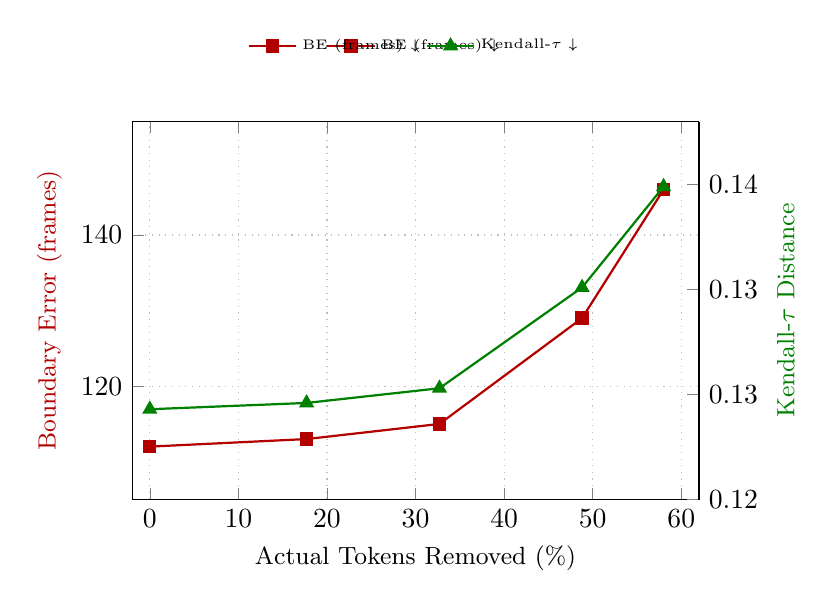
\begin{tikzpicture}
\pgfplotsset{scale only axis}

% -------------------------------------------------------------
% PRIMARY AXIS (Left): Boundary Error (BE)
% -------------------------------------------------------------
\begin{axis}[
    width=7.2cm,
    height=4.8cm,
    xlabel={Actual Tokens Removed (\%)},
    ylabel={Boundary Error (frames)},
    xmin=-2, xmax=62,
    ymin=105, ymax=155,
    axis y line*=left,
    y label style={font=\small, color=red!70!black},
    x label style={font=\small},
    tick label style={font=\xs},
    grid=major,
    grid style={dotted, gray!50},
    legend style={
        at={(0.5, 1.15)},
        anchor=south,
        legend columns=2,
        font=\tiny,
        draw=none,
        fill=none
    }
]

\addplot[color=red!70!black, mark=square*, thick, mark size=2pt] coordinates {
    (0.0, 112)
    (17.7, 113)
    (32.7, 115)
    (48.8, 129)
    (58.0, 146)
};
\addlegendentry{BE (frames) $\downarrow$}

\end{axis}

% -------------------------------------------------------------
% SECONDARY AXIS (Right): Kendall-tau Distance
% -------------------------------------------------------------
\begin{axis}[
    width=7.2cm,
    height=4.8cm,
    xmin=-2, xmax=62,
    hide x axis,
    ylabel={Kendall-$\tau$ Distance},
    ymin=0.120, ymax=0.138,
    axis y line*=right,
    y label style={font=\small, color=green!50!black},
    tick label style={font=\xs},
    legend style={
        at={(0.5, 1.15)},
        anchor=south,
        legend columns=2,
        font=\tiny,
        draw=none,
        fill=none
    }
]

% Legend dummy entry for left-axis metric
\addlegendimage{color=red!70!black, mark=square*, thick, mark size=2pt}
\addlegendentry{BE (frames) $\downarrow$}

\addplot[color=green!50!black, mark=triangle*, thick, mark size=2.4pt] coordinates {
    (0.0, 0.1243)
    (17.7, 0.1246)
    (32.7, 0.1253)
    (48.8, 0.1301)
    (58.0, 0.1349)
};
\addlegendentry{Kendall-$\tau \downarrow$}

\end{axis}

\end{tikzpicture}
\caption{Effect of token pruning rate (\texttt{max\_length}=4) on Boundary Error (BE) and Kendall-$\tau$ distance on the \texttt{NOTSOFAR DEV} benchmark[cite: 5]. Both metrics remain stable up to $\sim 33\%$ actual removal before degradation accelerates[cite: 5].}
\label{fig:notsofar_token_removal}
\end{figure}
\section{Conclusion}
We developed a number of algorithms to enable efficient long-form alignment of multi-talker transcripts, specifically analyzing the improvements made possible by incorporating speaker information during alignment. On long-form recordings, speaker information was not as helpful, however, on out-of-domain 30\,s recordings, speaker information modestly improved all alignment metrics. Speaker attribution performance of 17.6\% WDER is considerably better than the majority speaker baseline. All models are publicly released and we hope will facilitate the preparation and analysis of speaker attributed and transcribed multi-talker data. 
%\section{Acknowledgements}


% References should be produced using the bibtex program from suitable
% BiBTeX files (here: strings, refs, manuals). The IEEEbib.bst bibliography
% style file from IEEE produces unsorted bibliography list.
% -------------------------------------------------------------------------
\bibliographystyle{IEEEbib}
\bibliography{refs_compact_ieee_etal}

\end{document}
